\chapter{Hardware Implementation of the Proposed Algorithms}
\label{Implementation}

\section{Introduction}
This chapter presents the detailed hardware architectures developed for each FFT algorithm. It provides an in-depth analysis of critical design choices, including Block RAM (BRAM) allocation, DSP block utilization, delay register configuration, and pipelining strategies. Finally, it evaluates how these architectural decisions directly impact overall hardware resource utilization and computational latency.

\section{Shared Architectural Elements}
Before examining each algorithm individually, it is necessary to outline the design choices that are universally applied across all three implementations. Specifically, these shared architectural elements include the generation of twiddle factors, datapath optimization  to minimize resource consumption, the application of different complex multipliers architectures and the datatypes used.

\subsection{Twiddle Factors}
Because the proposed hardware implementations are designed for FFTs of fixed sizes (although the underlying RTL is parameterizable, the synthesized modules target specific sizes), there is no need to compute twiddle factors dynamically at runtime. Calculating these rotational coefficients involves trigonometric operations that are computationally expensive and consume valuable FPGA logic resources. To optimize efficiency, all twiddle factors are precomputed at compile time and statically stored in on-chip memory.

Given that certain FFT architectures require simultaneous access to multiple twiddle factors, the choice of memory architecture is critical. The memory must provide sufficient read bandwidth to prevent stalling the datapath. To meet these high-throughput requirements, twiddle factors are implemented using read-only distributed memory (such as LUTRAM or dedicated flip-flops). This guarantees single-cycle, constant-time access, ensuring that the computational units can retrieve the required constants without delay.

For example, the Radix-4 algorithm requires three distinct twiddle factors simultaneously for each butterfly computation. Attempting to store these coefficients in BRAM would be highly inefficient and structurally limiting, as BRAM primitives are strictly restricted to dual-port (two-read) operations. In contrast, distributed read-only memory supports multi-port parallel reads and synthesizes very efficiently within the general FPGA logic fabric.

\begin{figure}[H]
    \centering
    \begin{subfigure}[t]{0.48\linewidth}
        \centering
        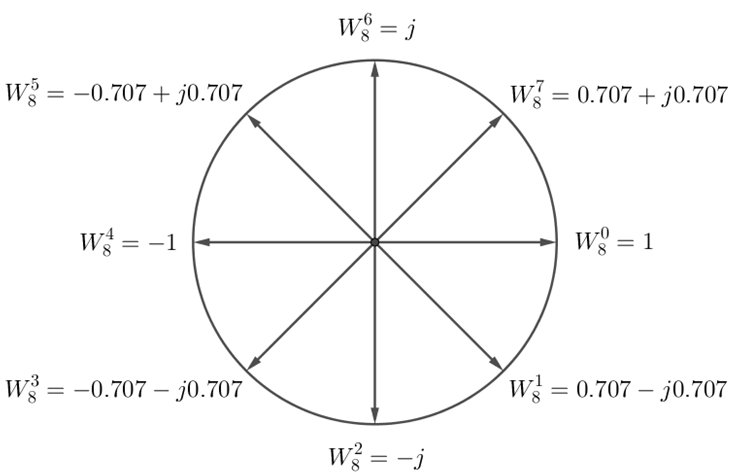
\includegraphics[width=\linewidth]{Images/cyrcle_2.png}
        \caption{Twiddle factors for N=8 represented on the unit circle.}
        \label{fig:twiddle_circle}
    \end{subfigure}
    \hfill
    \begin{subfigure}[t]{0.48\linewidth}
        \centering
        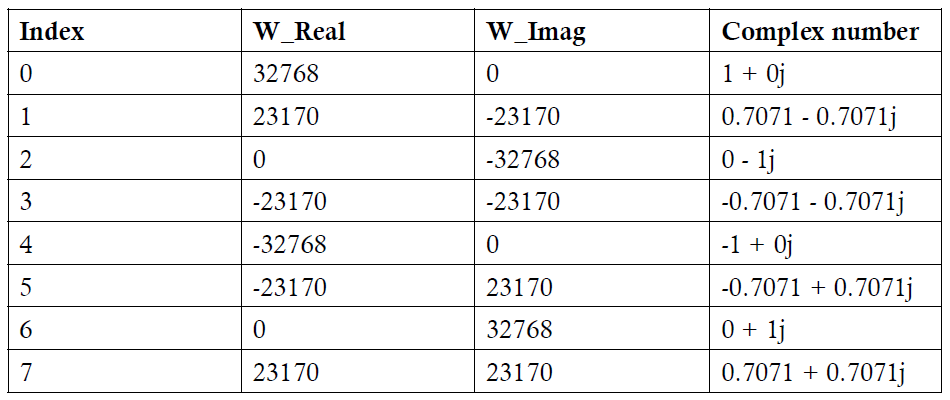
\includegraphics[width=\linewidth]{Images/tw.png}
        \caption{Twiddle values for N=8.}
        \label{fig:twiddle_values}
    \end{subfigure}
    \caption{Twiddle factor visualization.}
\end{figure}

The twiddle factors are generated by sampling the complex exponential function, $W_N = e^{-j\frac{2\pi}{N}}$, at $N$ discrete intervals, where $N$ represents the size of the FFT. These ideal floating-point values are subsequently quantized to match the target fixed-point resolution used in the hardware datapath.

The intuitive approach to storing twiddle factors would be to utilize a single, centralized memory shared across all FFT stages. However, this is architecturally impractical for a highly pipelined design. First, standard BRAM primitives lack the multi-port capabilities required for simultaneous multi-stage access. Second, implementing a centralized memory using read-only LUTRAMs would require extensive logic replication to achieve the necessary read bandwidth, completely defeating the purpose of a unified memory structure.Consequently, the design employs a distributed memory architecture, allocating a dedicated memory module to each individual FFT stage. However, because different stages require different subsets of the twiddle factors, duplicating the entire $N$-point coefficient array at every stage would be highly inefficient. To optimize resource utilization, a custom generation script was developed that mimics the algorithmic dataflow of the FFT. This script precomputes and generates customized, stage-specific memory modules that contain only the exact coefficients required for that particular stage, drastically minimizing the overall memory footprint.

\begin{table}[htbp]
    \centering
    \caption{Comparison of twiddle factor memory footprint between a naive duplicated storage approach and the proposed stage-specific optimized generation for an 8-stage Radix-2 FFT (DIT).}
    \vspace{0.5em}
    \begin{tabular}{|c|c|c|}
        \hline
        \textbf{FFT Stage} & \textbf{Naive Storage (Duplicated)} & \textbf{Optimized Storage} \\
        \hline
        Stage 1 & 128 & 1 \\
        Stage 2 & 128 & 2 \\
        Stage 3 & 128 & 4 \\
        Stage 4 & 128 & 8 \\
        Stage 5 & 128 & 16 \\
        Stage 6 & 128 & 32 \\
        Stage 7 & 128 & 64 \\
        Stage 8 & 128 & 128 \\
        \hline
        \textbf{Total Twiddle Factors} & \textbf{1024} & \textbf{255} \\
        \hline
    \end{tabular}
    \label{tab:twiddle_memory_comparison}
\end{table}

This works similarly for the rest of the algorithms

\subsection{Datapaths}
It is important to note that non-critical datapath registers are implemented without a hardware reset signal. This alleviates routing congestion across the FPGA fabric and theoretically enables the synthesis tool to achieve better timing and resource optimization.

\subsection{Datatypes}
Because the FFT processor is designed with parameterizable resolution, the datapath word length is dynamically determined by the selected twiddle factor size. This size establishes the $Q1.x$ fixed-point format for the system, where $x$ represents the fractional bit width. The input data, assumed to be normalized within the range $(-1, 1)$, is initially quantized to this baseline resolution. However, as the data propagates through the core, the arithmetic operations within the butterfly units naturally expand the required bit width.

A common technique to manage this expansion is to scale down or truncate the output at each stage to maintain a strictly constant word length. However, this approach severely degrades the computational accuracy of the processor, particularly for high-order FFTs, resulting in a Signal-to-Quantization-Noise Ratio (SQNR) degradation of approximately 6 dB per additional stage \cite{garcia2007fpga}.

To preserve numerical precision while remaining scalable to large transform sizes, the proposed architecture employs a progressive bit-growth strategy. The datapath width is allowed to increase at each stage to accommodate the exact number of sequential additions within the butterfly unit, guaranteeing overflow protection. For complex multiplications, the intermediate products are truncated to retain only the most significant bits (MSBs) corresponding to the established data width, balancing high precision with efficient hardware utilization.

\subsection{Complex Multiplication Techniques}

To provide flexibility in resource management, the proposed architecture is parameterizable, allowing the design to choose between two distinct complex multiplication techniques: the traditional direct method and the Gauss 3-multiplier method.

Let the complex input data be $A = a_{re} + j a_{im}$ and the complex twiddle factor be $W = w_{re} + j w_{im}$. The resulting complex product is $P = p_{re} + j p_{im}$.

\textbf{Traditional Complex Multiplication} \\
The traditional approach computes the complex product through direct algebraic expansion. The real and imaginary components are calculated as:
\begin{align}
    p_{re} &= a_{re}w_{re} - a_{im}w_{im} & p_{im} &= a_{re}w_{im} + a_{im}w_{re} \label{eq:trad_mult}
\end{align}
This implementation requires exactly four separate multiplication operations and two additions/subtractions. In hardware, this directly translates to four DSP blocks per complex multiplier unit.

\textbf{Gauss 3-Multiplier Technique} \\
To reduce the dependency on DSP blocks, the design implements the Carl Friedrich Gauss complex multiplication algorithm. By algebraically factoring the equations, this technique trades one multiplication for three additional addition operations.

First, three intermediate addition and subtraction values are precomputed:
\begin{align}
    S_a &= a_{re} + a_{im} & S_w &= w_{re} + w_{im} & D_w &= w_{im} - w_{re}
\end{align}
Next, three partial products ($m_1, m_2, m_3$) are generated using only three multipliers:
\begin{align}
    m_1 &= w_{re} \cdot S_a & m_2 &= a_{re} \cdot D_w & m_3 &= a_{im} \cdot S_w
\end{align}
Finally, the real and imaginary components of the product are assembled using two final additions:
\begin{align}
    p_{re} &= m_1 - m_3 & p_{im} &= m_1 + m_2
\end{align}
While this architecture increases the adder count to five, it successfully reduces the multiplier count to three. This translates in a 25\% reduction in DSP utilization per multiplier.

\section{Radix-2 Implementation}
\subsection{Review of Prior Implementation}
The initial implementation of an FFT processor was developed as a collaborative project during a Microprocessor Design course. This architecture consisted of a baseline Radix-2 Single-Path Delay Feedback (SDF) core, designed without pipelining and operating with a throughput of one sample per stage and a data width of 32 bit with a Q1.15 quantization. The synthesis results for this legacy design are presented in the following table. Rather than focusing on the physical area of the design, this comparison emphasizes the critical path and overall processing latency. Both of these performance metrics see significant improvements in the  implementations shown later in this work, by pipelining and increasing throughput.

\begin{table}[htbp]
    \centering
    \caption{Synthesis results and latency for the baseline 256-point FFT architecture.}
    \vspace{0.5em}
    \begin{tabular}{lc}
        \hline
        \textbf{Metric} & \textbf{FFT-256} \\
        \hline
        Critical Path (ns) & 13.976 \\
        LUTs & 3161 \\
        Registers & 1576 \\
        DSPs & 56 \\
        Latency (clock cycles) & 259 \\
        \hline
    \end{tabular}
    \label{tab:baseline_results_256}
\end{table}

\subsection{Overview of Proposed Implementation}
In the new implementation, the throughput is increased from one to two samples per clock cycle. Additionally, the design incorporates extensive pipelining, with a particular focus on the internal datapath of the butterfly unit to reduce the critical path delay. The processor employs a Decimation-in-Time (DIT) architecture, which inherently requires the input data to be supplied in bit-reversed order while generating outputs in natural sequential order. Its counterpart, the Decimation-in-Frequency (DIF) architecture, operates conversely by accepting natural-order inputs and producing bit-reversed outputs. Because both algorithms share the same computational complexity and hardware requirements, the decision to implement a DIT rather than a DIF processor is primarily dictated by the specific data sequencing constraints and integration requirements of the broader system.

\subsection{Butterfly Radix-2}

Algorithm \ref{alg:radix2_butterfly} shows the operational flow of the RTL implementation for the pipelined butterfly unit. The process begins with the complex multiplication of input $B$ and the twiddle factor $W$, utilizing one of the two selectable multiplier architectures. To ensure correct alignment for the final butterfly computation, adjustable delay registers synchronize input $A$ with the latency of the multiplication stage. In the final phase, the product is scaled to the target word length before executing the cross-over addition and subtraction operations. Concurrently, a valid signal is propagated through a matching delay pipeline to flag output readiness. Lastly, in the first stage of any Radix-2 FFT, the twiddle factor is strictly $W = 1 + j0$. The architecture uses this mathematical property by replacing the complex multiplier with a trivial bit-shift.

Analyzing the arithmetic operations within the butterfly module, it is evident that the required bit growth between stages is 1 bit due to the single addition performed at the end of the butterfly.

\begin{algorithm}[H]
\caption{Pipelined Radix-2 Butterfly}
\label{alg:radix2_butterfly}
\begin{algorithmic}[1]
\Require Complex inputs $A$, $B$; twiddle factor $W$; $start$ signal
\Ensure  Complex outputs $Out_1$, $Out_2$; $done$ signal

\Statex \textbf{Step 1: Complex multiplication of $B$ by $W$}
\If{$\mathit{stage} = 1$}
    \State $B_{\mathit{mult}} \gets B \ll (\mathit{Tw\_Width} - 1)$
           \Comment{$W = 1$: shift replaces the multiplier}
\ElsIf{$\mathit{SimpleMult} = 1$}
    \State $B_{\mathit{mult}} \gets \Call{TraditionalComplexMult}{B, W}$
           \Comment{4 mult, 2 add}
\Else
    \State $B_{\mathit{mult}} \gets \Call{GaussComplexMult}{B, W}$
           \Comment{3 mult, 5 add}
\EndIf

\Statex \textbf{Step 2: Pipeline balancing}
\State $A_{\mathit{delayed}} \gets \Call{Delay}{A, L_{\mathit{mult}}}$
       \Comment{match multiplier latency}
\State $done \gets \Call{Delay}{start, L_{\mathit{total}}}$
       \Comment{match total pipeline latency}

\Statex \textbf{Step 3: Scaling and butterfly}
\State $B_{\mathit{scaled}} \gets \Call{Truncate}{B_{\mathit{mult}}, \mathit{Tw\_Width} - 1}$
       \Comment{remove twiddle scaling}
\State $Out_1 \gets A_{\mathit{delayed}} + B_{\mathit{scaled}}$
\State $Out_2 \gets A_{\mathit{delayed}} - B_{\mathit{scaled}}$
\end{algorithmic}
\end{algorithm}
% Place this inside your document where you want the algorithm to appear:


\subsection{First Stage}

\begin{figure}[H]
    \centering
    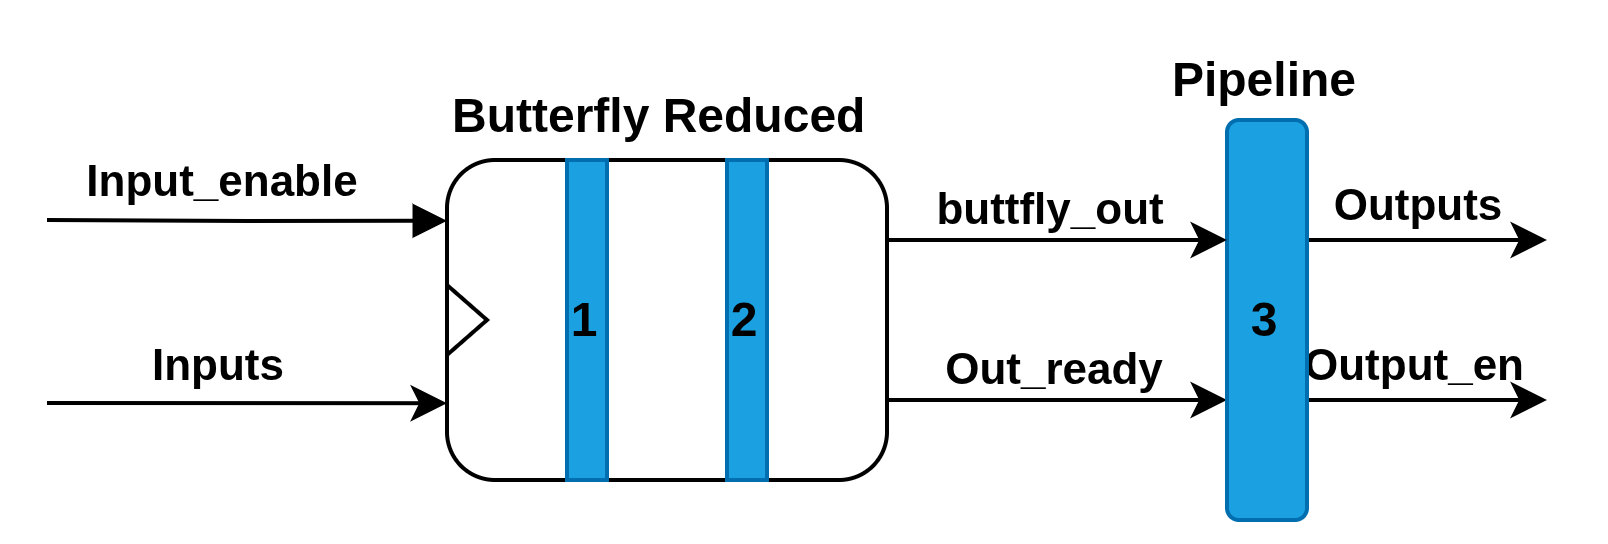
\includegraphics[width=0.8\textwidth]{Images/Stage_1.drawio.png} 
    \caption{Radix-2 fisrt stage top module.}
    \label{fig:Stage_1_r2}
\end{figure}

The first stage is the simplest part of the processor design. Not only is the butterfly unit itself simplified, but the overall stage requires less hardware because no delay registers are needed to align the input data. This can be seen in the far-left stage of the Radix-2 dataflow in Figure \ref{fig:FFT_dataflows}. As a result, the hardware for this first stage consists entirely of just the simplified butterfly unit.

\subsection{Control Unit}
The control unit is responsible for coordinating where inputs are stored, when butterfly operations start, and how the delay buffers function. This is achieved using two counters of variable size, which depends on the stage number.

The first is the \textit{stride segment counter}, which times the writing of new inputs to memory and tracks when the second counter should start. This counter increments every time four new samples arrive (shown as green lines in the graphs).

The second is the \textit{butterfly operation counter}, which starts when the samples required for the butterfly operation arrive. These are the blue samples in the graph, they represent the last samples of a butterfly cluster needed to complete the set of four inputs. Since only one physical butterfly unit exists, we cannot process all four operations at once even if we have the data. Therefore, only one operation happens at a time, and the other data must wait.

To make the design simpler and more portable, these counters do not iterate through all operations in a stage. Instead, each counter counts up to the number of butterflies in the respective cluster (in the graph, this number is 2). The length of these counters is calculated dynamically based on parameters from the SDF unit module that indicate the current stage.

Finally, there are other signals, such as the butterfly counter enable, which validates that the inputs and outputs of the butterfly are valid. There is also a flush counter that tracks the number of remaining operations when the input enable signal goes low. This is needed because the unit requires extra time to finish processing after the last input is received due to the initial delay while waiting for values to arrive.

\begin{figure}[H]
    \centering
    % --- First Row ---
    \begin{subfigure}[b]{0.48\linewidth}
        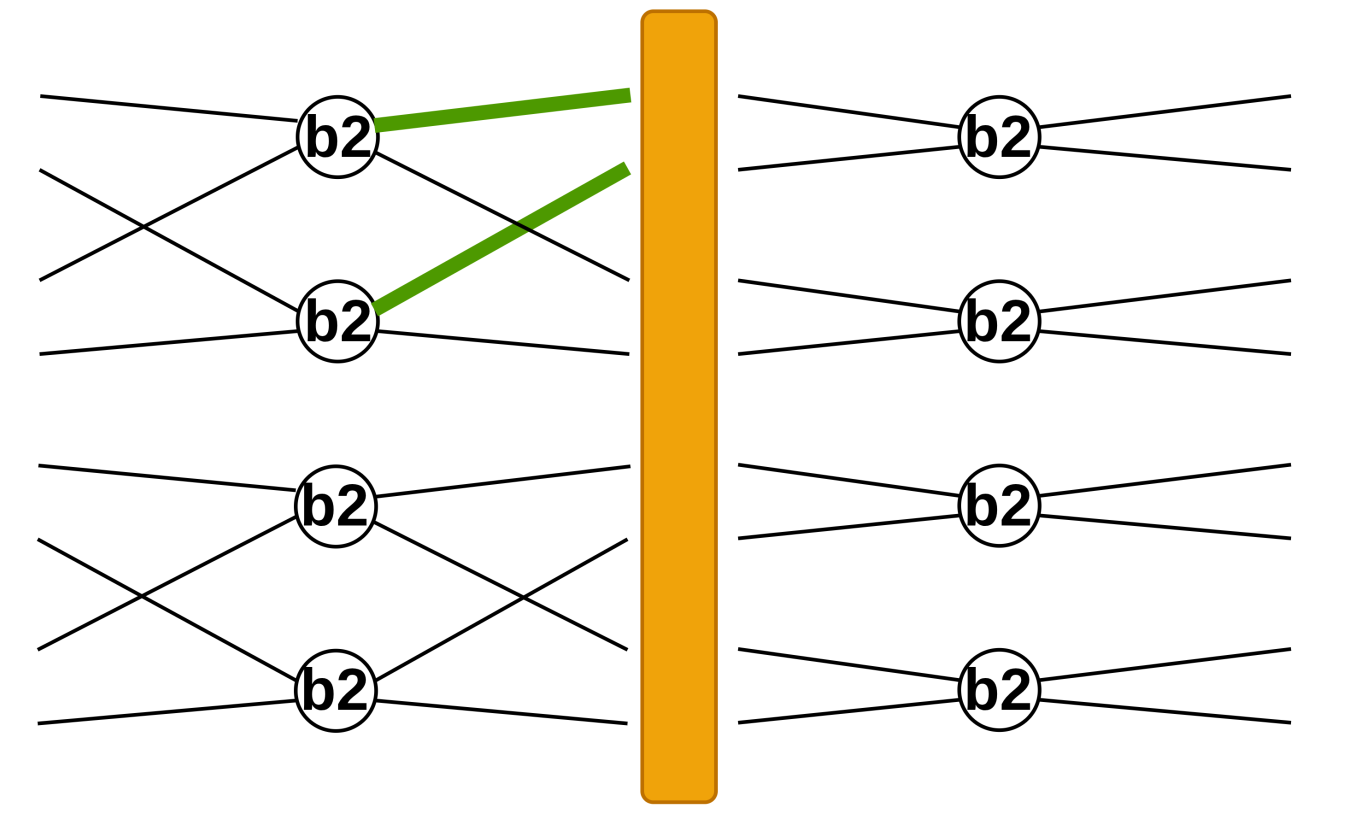
\includegraphics[width=\linewidth]{Images/Control_r2_1.png}
        \caption{Stride counter equals 0}
        \label{fig:tetrada1}
    \end{subfigure}
    \hfill
    \begin{subfigure}[b]{0.48\linewidth}
        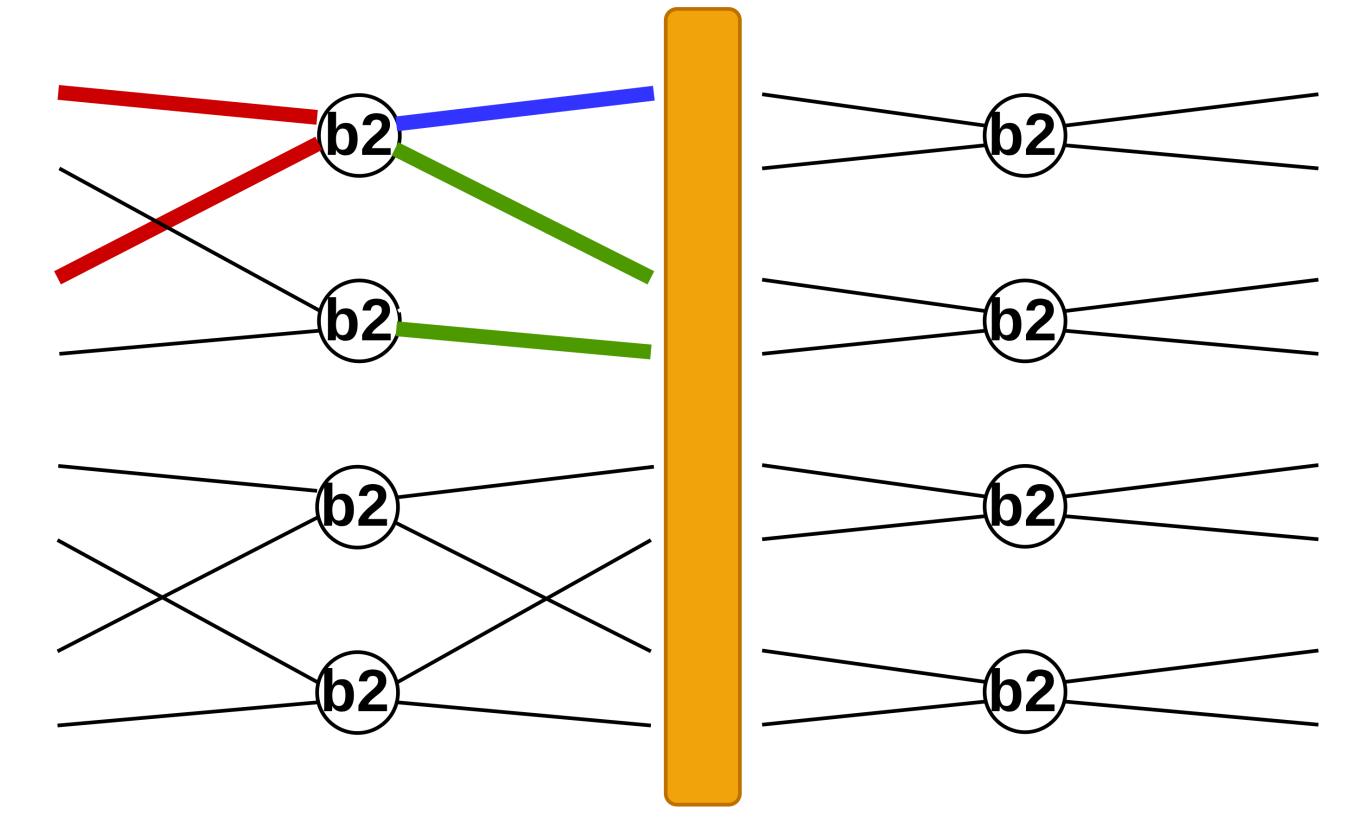
\includegraphics[width=\linewidth]{Images/Control_r2_2.png}
        \caption{Stride counter equals 1 butterfly counter 0}
        \label{fig:tetrada2}
    \end{subfigure}
    
    \vspace{1em}
    
    % --- Second Row ---
    \begin{subfigure}[b]{0.48\linewidth}
        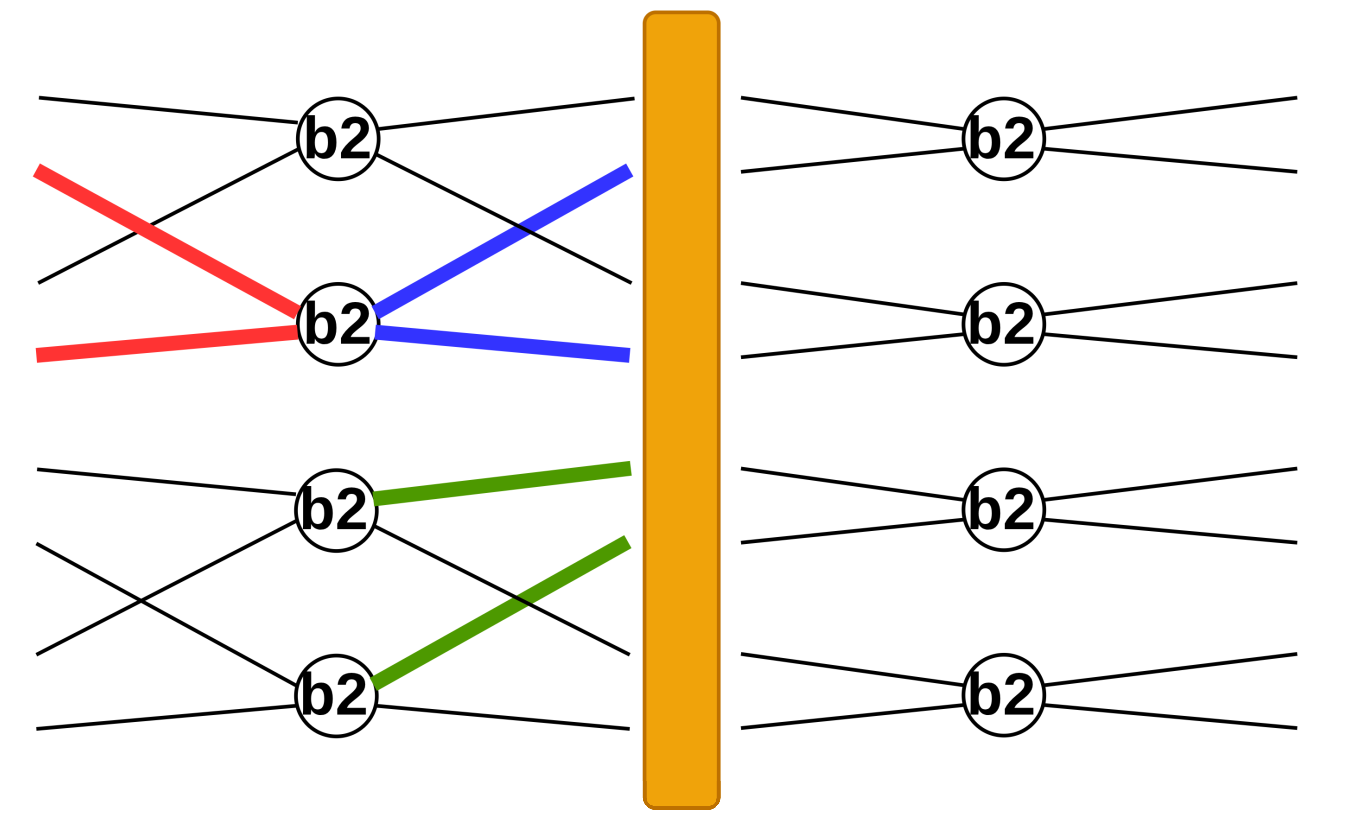
\includegraphics[width=\linewidth]{Images/Control_r2_3.png}
        \caption{Stride counter equals 0, butterfly counter 1}
        \label{fig:tetrada3}
    \end{subfigure}
    \hfill
    \begin{subfigure}[b]{0.48\linewidth}
        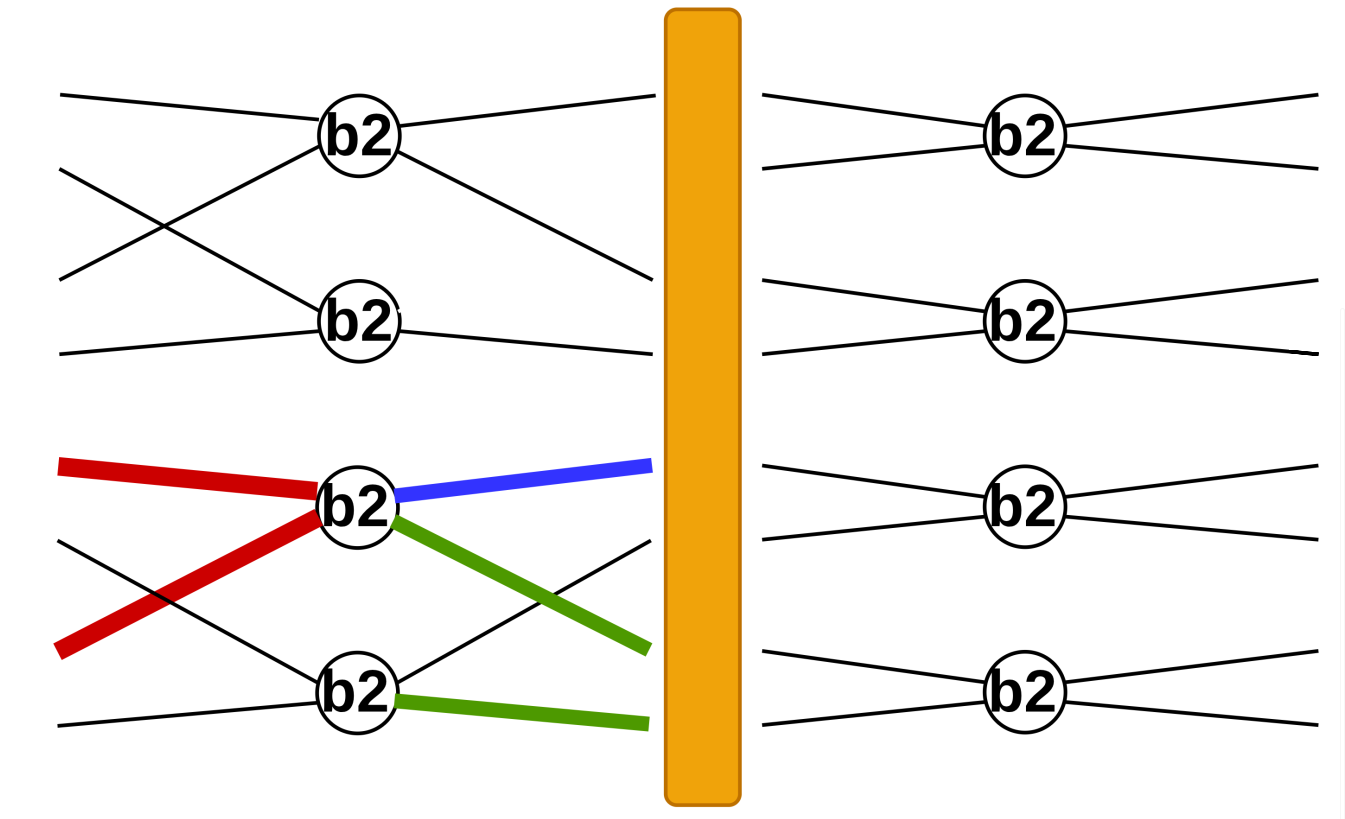
\includegraphics[width=\linewidth]{Images/Control_r2_4.png}
        \caption{Stride counter equals 1, butterfly counter 0}
        \label{fig:tetrada4}
    \end{subfigure}
    
    \caption{Operation flow of the counters managing the pairs of data points.}
    \label{fig:all_tetradas}
\end{figure}

\subsection{Delay Registers and Final Design}
To properly align the incoming data, it must be stored temporarily. We achieve this by using simple delay buffers with an adjustable (parameterizable) depth. This allows the same buffer design to be reused across all stages, even though each stage requires a different latency.

For this design, only two delay registers are needed per stage. Their depths are calculated as:
\begin{itemize}
    \item $\mathrm{Depth\_A} = 2^{\mathrm{STAGE\_NUM} - 1}$ 
    \item $\mathrm{Depth\_B} = \mathrm{Depth\_A} \times 2$
\end{itemize}

Because the buffer depth doubles with each additional stage, the overall hardware area increases exponentially for larger FFT sizes. With the addition of these delay registers, the Stage module is complete. In the diagram, the output dataflow pipelines are highlighted in blue, and the input dataflow pipelines are highlighted in green.

\begin{figure}[H]
    \centering
    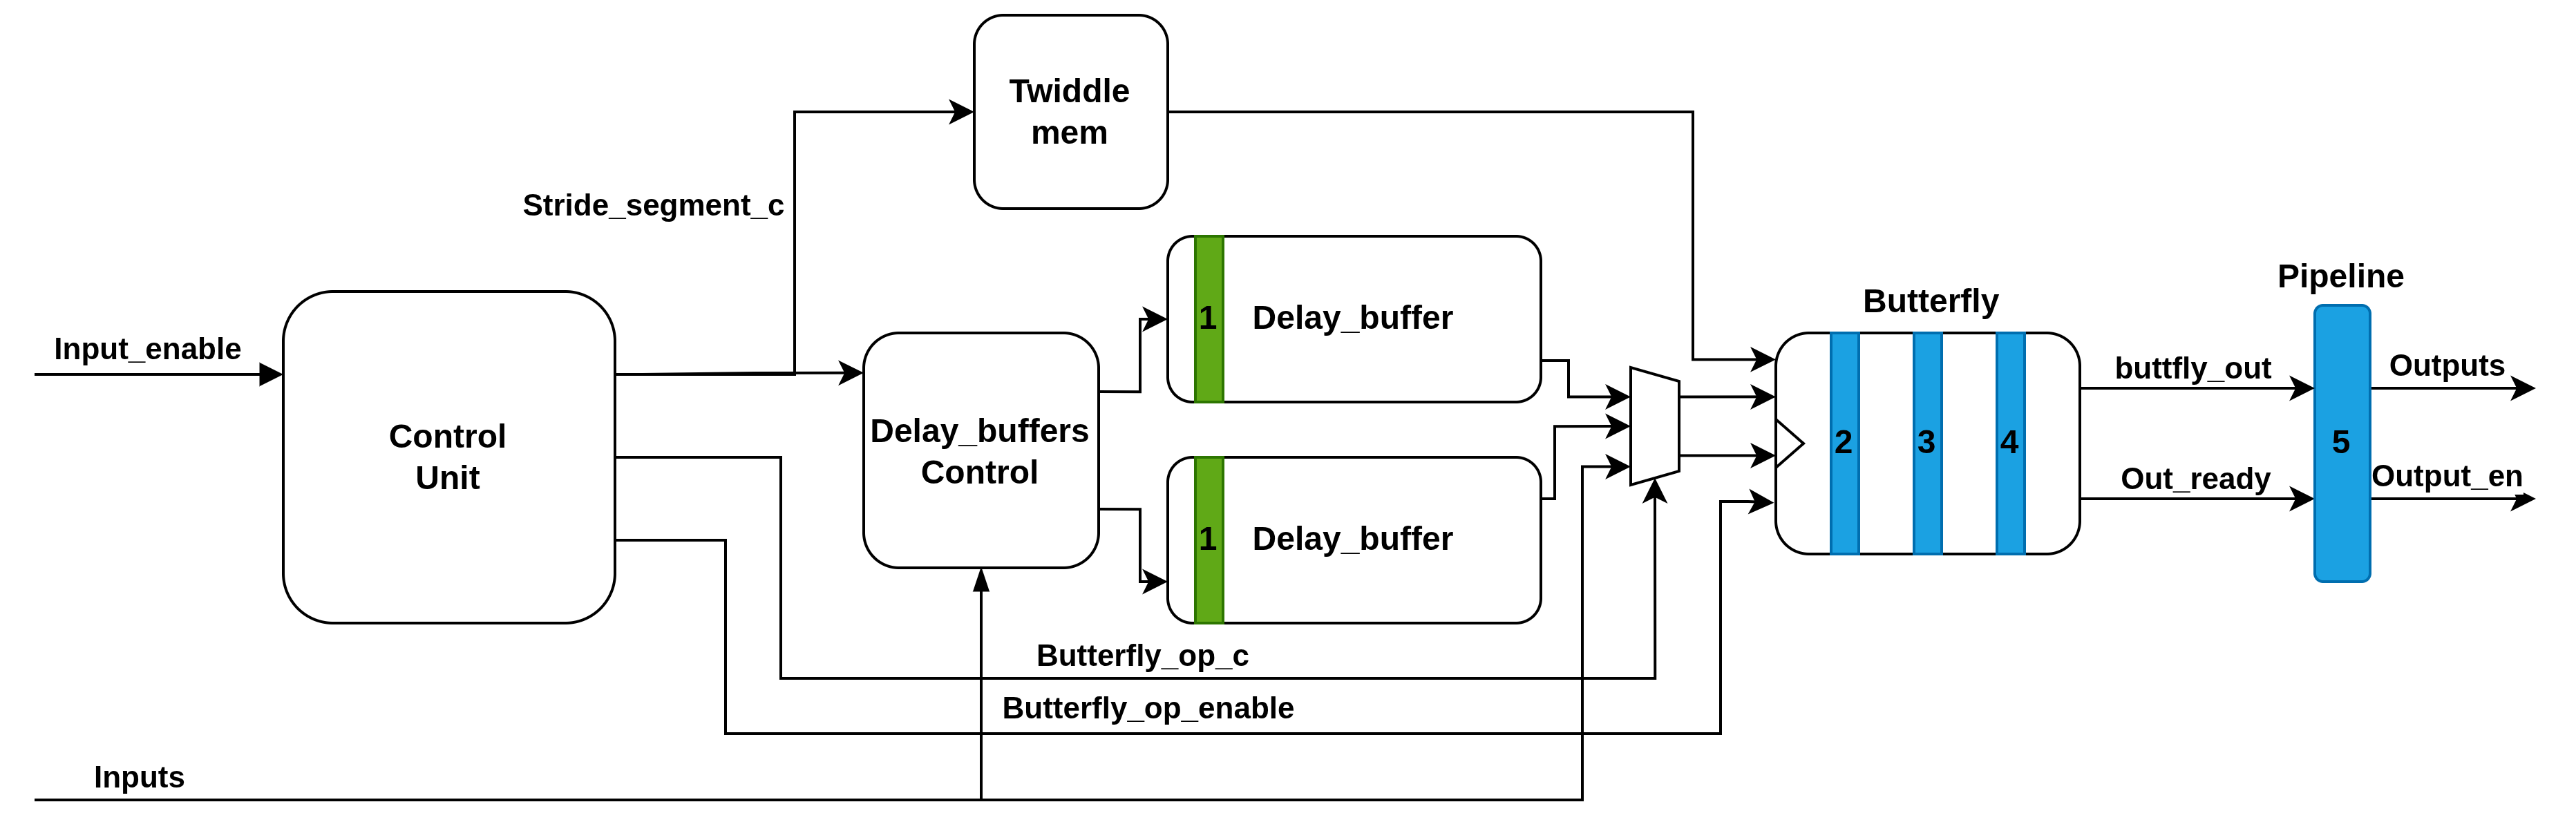
\includegraphics[width=1\textwidth]{Images/Radix-2_stage_unit.drawio.png} 
    \caption{Radix-2 general stage unit top module.}
    \label{fig:Stage_1_r2}
\end{figure}

In the top-level module, which connects all stage units to form a complete FFT, each stage's outputs are chained directly to the next stage's inputs. The first stage receives the input samples, and the final stage produces the results.

To accommodate bit growth, each stage instantiation can have a different data width. The top module calculates the maximum required bit width based on the input parameters, and the RTL dynamically scales the bit width for the specific stages that require it. For example, if the starting parameters specify a data width of 14 and a twiddle width of 10, the top module will only begin increasing the bit size after the fourth stage.

Because unoptimized widths can waste resources, the general rule for this design is that the starting data width should be equal to the twiddle width plus one. This constraint is not enforced automatically in the RTL solely to provide greater flexibility for testing and simulating the design.

\subsection{Implementation Results using an ISO Clock}
These implementations utilize a generous clock frequency of 100 MHz (a 10 ns clock period) and an 8-bit twiddle factor width to highlight the area differences between the implemented algorithms on an Artix-7 AC701 Evaluation Platform (\texttt{xc7a200tfbg676-2}). Furthermore, only powers-of-four FFT sizes are presented to ensure direct comparability with subsequent radix-4 designs.

\begin{figure}[H]
    \centering
    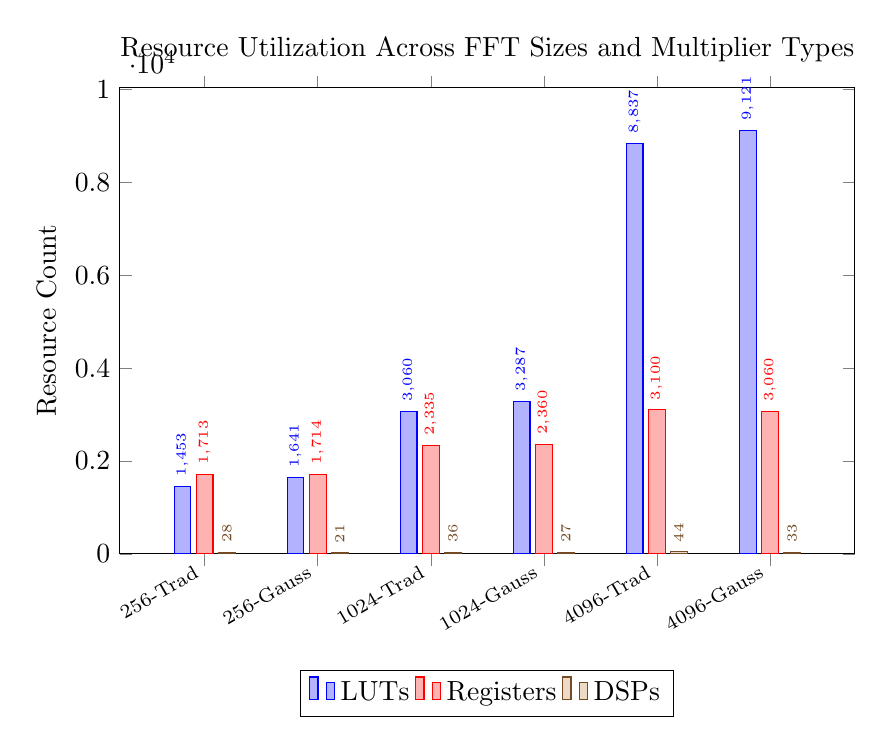
\begin{tikzpicture}
        \begin{axis}[
            ybar,
            width=0.9\textwidth,
            height=7.5cm,
            ylabel={Resource Count},
            symbolic x coords={256-Trad, 256-Gauss, 1024-Trad, 1024-Gauss, 4096-Trad, 4096-Gauss},
            xtick=data,
            x tick label style={rotate=30, anchor=east, font=\scriptsize},
            nodes near coords,
            every node near coord/.append style={font=\tiny, rotate=90, anchor=west},
            legend style={at={(0.5,-0.25)}, anchor=north, legend columns=-1},
            title={Resource Utilization Across FFT Sizes and Multiplier Types},
            ymin=0,
            enlarge x limits=0.15,
            bar width=6pt,
        ]
            % LUTs
            \addplot coordinates {
                (256-Trad, 1453) (256-Gauss, 1641) 
                (1024-Trad, 3060) (1024-Gauss, 3287) 
                (4096-Trad, 8837) (4096-Gauss, 9121)
            };
            
            % Registers
            \addplot coordinates {
                (256-Trad, 1713) (256-Gauss, 1714) 
                (1024-Trad, 2335) (1024-Gauss, 2360) 
                (4096-Trad, 3100) (4096-Gauss, 3060)
            };
            
            % DSPs
            \addplot coordinates {
                (256-Trad, 28) (256-Gauss, 21) 
                (1024-Trad, 36) (1024-Gauss, 27) 
                (4096-Trad, 44) (4096-Gauss, 33)
            };
            
            \legend{LUTs, Registers, DSPs}
        \end{axis}
    \end{tikzpicture}
    \caption{Utilization comparison (LUTs, Registers, and DSPs) for Radix-2 FFT implementations across sizes 256, 1024, and 4096 under ISO clock constraints.}
    \label{fig:radix2_all_resources_combined}
\end{figure}

\begin{table}[H]
    \centering
    \caption{FIFO Radix-2 Latency.}
    \vspace{0.5em}
    \begin{tabular}{lcccc}
        \hline
        \textbf{Metric} & \textbf{New-256} & \textbf{New-1024} & \textbf{New-4096} & \textbf{New-256} \\
        \hline
        Latency Trad (cycles) & 165 & 559 & 2105 & 259 \\
        Latency Gauss (cycles) & 172 & 568 & 2116 & -- \\
        \hline
    \end{tabular}
    \label{tab:baseline_results_256}
\end{table}

Due to the registers used for data alignment, the register growth for 4096 samples is substantial, and a closer inspection reveals that it doubles with each successive increase in FFT size. Furthermore, a comparison between the legacy 256-point and new 256-point FFT implementations shows a reduction in overall latency. Although the throughput is doubled, the latency is not reduced by half; this is caused by the extra pipelining introduced in the new stage unit, which adds a constant cycle penalty but ultimately yields significantly better timing results.

\section{Radix-4 Implementation}

\subsection{Overview of Proposed Implementation}
For the implementation of the Radix-4 algorithm, a methodology similar to that of the Radix-2 design is adopted. The architecture is configured to achieve the maximum throughput supported by the Radix-4 butterfly (four samples per clock cycle), while exploring alternative buffering strategies to efficiently store and align the data. As with the preceding design, this implementation follows a Decimation-in-Time (DIT) structure, requiring the input sequence to be supplied in digit-reversed order (base-4 reversal).

\subsection{Butterfly Radix-4}
Algorithm \ref{alg:radix4_butterfly} operates similarly to the Radix-2 butterfly, but is adapted for Radix-4 arithmetic. It reuses the same multiplication techniques and requires delay registers to align the $A$ inputs with the outputs of the multipliers.

Analyzing the arithmetic operations within the butterfly module, it is evident that the required bit growth between stages is 2 bits, due to the two consecutive additions performed at the end of the butterfly.

\begin{algorithm}
\caption{Pipelined Radix-4 Butterfly}
\label{alg:radix4_butterfly}
\begin{algorithmic}[1]
\Require Complex inputs $A$, $B$, $C$, $D$; twiddle factors $W_0$, $W_1$, $W_2$; $start$ signal
\Ensure  Complex outputs $Out_1$, $Out_2$, $Out_3$, $Out_4$; $done$ signal

\Statex \textbf{Step 1: Complex multiplication of $B$, $C$, $D$ by $W_0$, $W_1$, $W_2$}
\If{$\mathit{stage\_num} = 1$}
    \State $B_{\mathit{mult}} \gets B \ll (\mathit{Tw\_Width} - 1)$ \Comment{Shift replaces multiplier}
    \State $C_{\mathit{mult}} \gets C \ll (\mathit{Tw\_Width} - 1)$ 
     $D_{\mathit{mult}} \gets D \ll (\mathit{Tw\_Width} - 1)$ 
\ElsIf{$\mathit{SimpleMult} = 1$}
    \State $B_{\mathit{mult}} \gets \Call{SimpleMult}{B, W_0}$ \Comment{Traditional complex multiplier}
    \State $C_{\mathit{mult}} \gets \Call{SimpleMult}{C, W_1}$ 
     $D_{\mathit{mult}} \gets \Call{SimpleMult}{D, W_2}$ 
\Else
    \State $B_{\mathit{mult}} \gets \Call{CheapMult}{B, W_0}$ \Comment{Gauss complex multiplier}
    \State $C_{\mathit{mult}} \gets \Call{CheapMult}{C, W_1}$
     $D_{\mathit{mult}} \gets \Call{CheapMult}{D, W_2}$ 
\EndIf

\Statex \textbf{Step 2: Pipeline balancing}
\State $A_{\mathit{delayed}} \gets \Call{Delay}{A, \mathit{delay\_mult} + 1}$ \Comment{Match multiplier latency + scale reg}
\State $done \gets \Call{Delay}{start, \mathit{delay\_mult} + 3}$ \Comment{Match total pipeline latency}

\Statex \textbf{Step 3: Scaling}
\State $B_{\mathit{scaled}} \gets \Call{Truncate}{B_{\mathit{mult}}, \mathit{Tw\_Width} - 1}$ \Comment{Remove twiddle scaling}
\State $C_{\mathit{scaled}} \gets \Call{Truncate}{C_{\mathit{mult}}, \mathit{Tw\_Width} - 1}$ 
\State $D_{\mathit{scaled}} \gets \Call{Truncate}{D_{\mathit{mult}}, \mathit{Tw\_Width} - 1}$ 

\Statex \textbf{Step 4: Butterfly Stage 1 (Intermediate variables)}
\State $t_0 \gets A_{\mathit{delayed}} + C_{\mathit{scaled}}$
\State $t_1 \gets A_{\mathit{delayed}} - C_{\mathit{scaled}}$
\State $t_2 \gets B_{\mathit{scaled}} + D_{\mathit{scaled}}$
\State $t_3 \gets B_{\mathit{scaled}} - D_{\mathit{scaled}}$

\Statex \textbf{Step 5: Butterfly Stage 2 (Outputs)}
\State $Out_1 \gets t_0 + t_2$
\State $Out_2 \gets t_1 - j \cdot t_3$ \Comment{Implemented as $t_{1r} + t_{3i}$ and $t_{1i} - t_{3r}$}
\State $Out_3 \gets t_0 - t_2$
\State $Out_4 \gets t_1 + j \cdot t_3$ \Comment{Implemented as $t_{1r} - t_{3i}$ and $t_{1i} + t_{3r}$}
\end{algorithmic}
\end{algorithm}

\subsection{First Stage}
\begin{figure}[H]
    \centering
    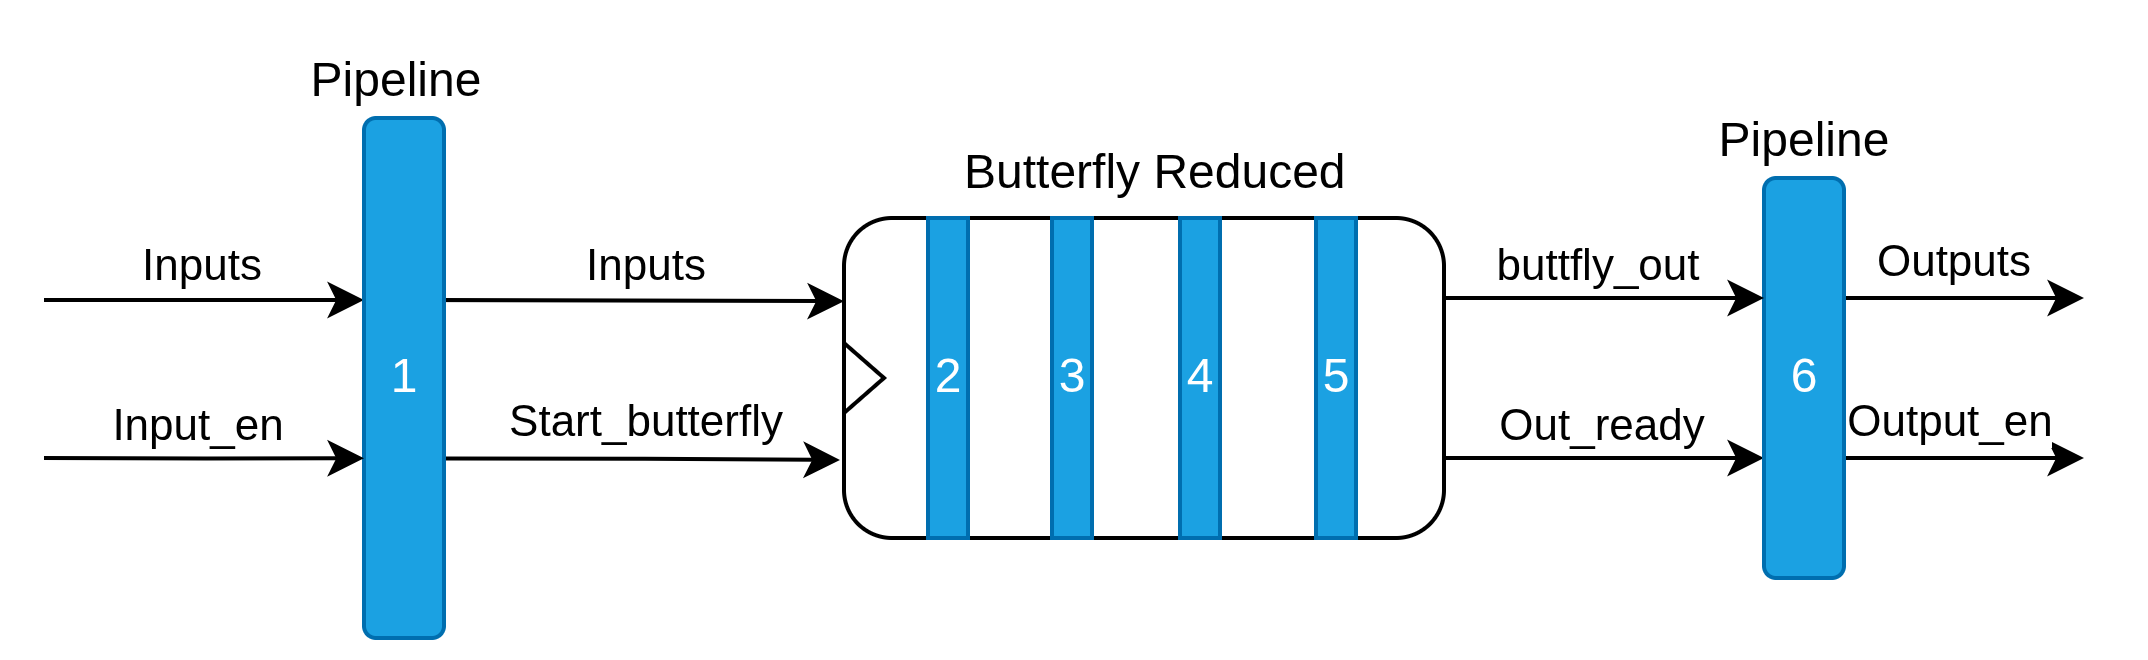
\includegraphics[width=0.8\textwidth]{Images/Stage_1_r4.drawio.png} 
    \caption{Radix-4 fisrt stage top module.}
    \label{fig:Stage_1_r2}
\end{figure}

The first stage is again the simplest part of the processor design.  The butterfly unit itself is simplified and the overall stage requires less hardware because no delay registers are needed to align the input data. This can be seen in the far-left stage of the Radix-4 dataflow in Figure \ref{fig:FFT_dataflows}. As a result, the hardware for this first stage consists entirely of just the simplified butterfly unit.

\subsection{Control Unit}
\begin{figure}[H]
    \centering
    % --- First Row ---
    \begin{subfigure}[b]{0.3\linewidth}
        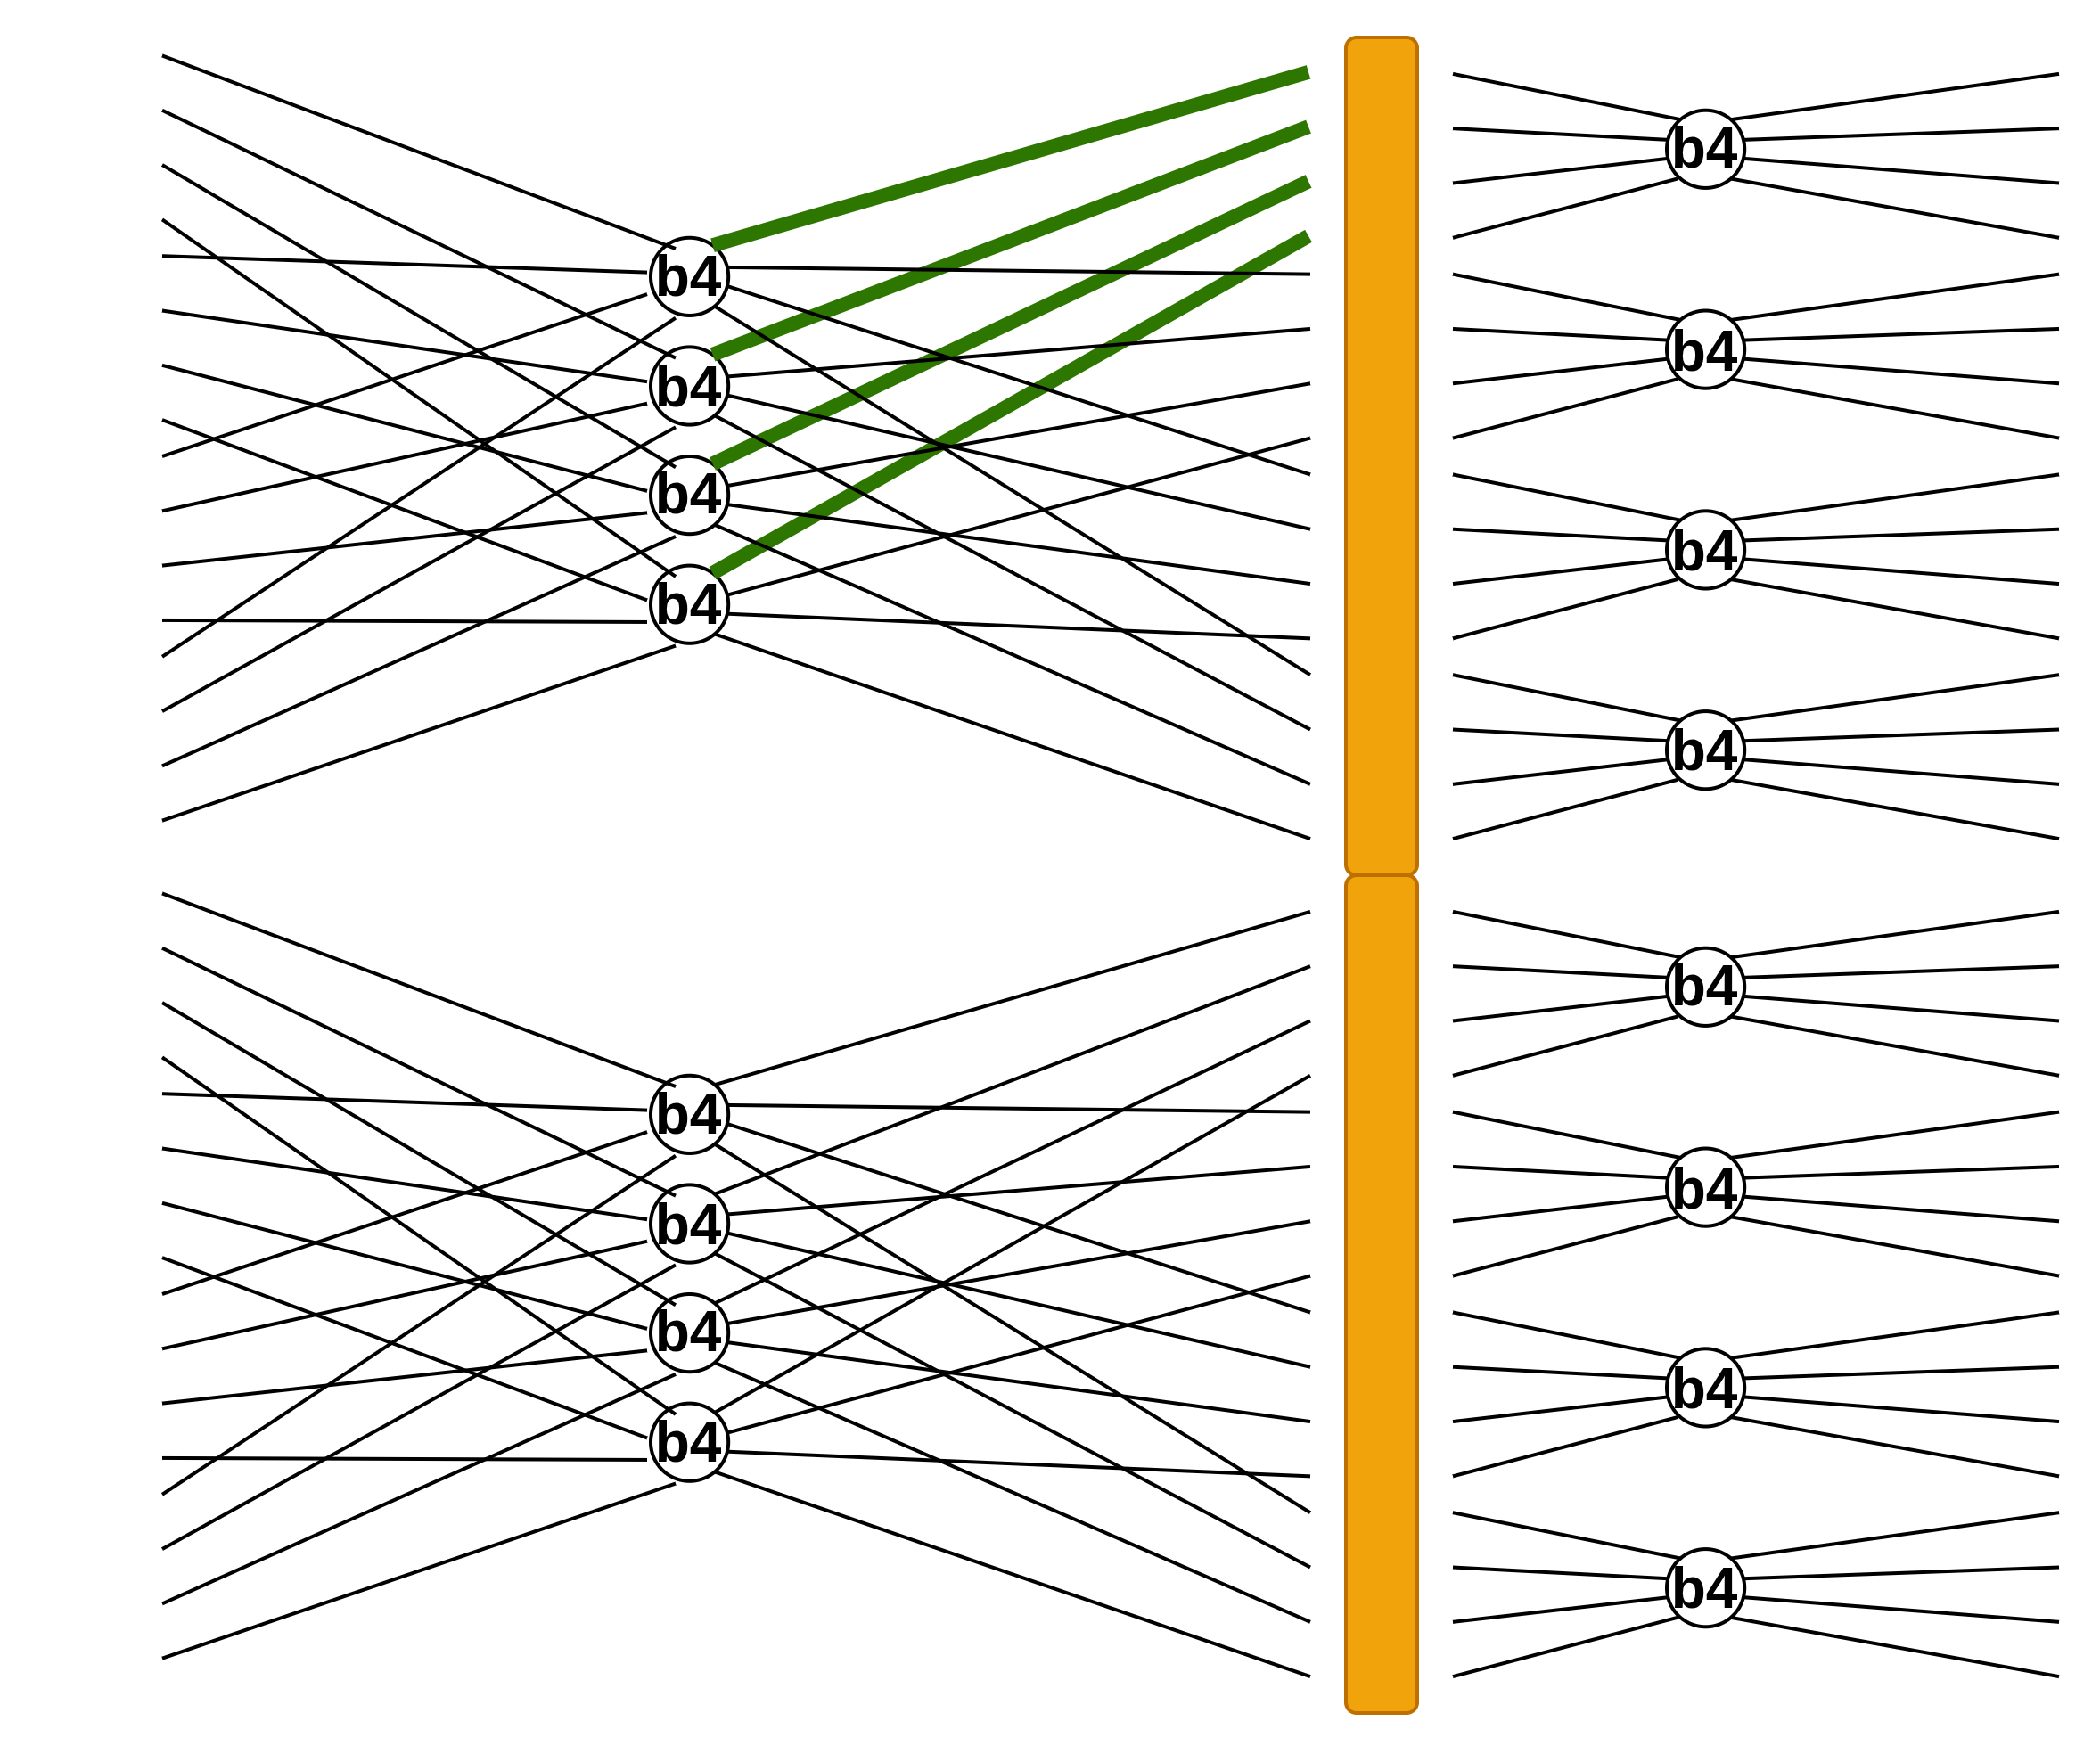
\includegraphics[width=\linewidth]{Images/1st_tetrada.png}
        \caption{Stride counter equals 00}
        \label{fig:tetrada1}
    \end{subfigure}
    \hfill
    \begin{subfigure}[b]{0.3\linewidth}
        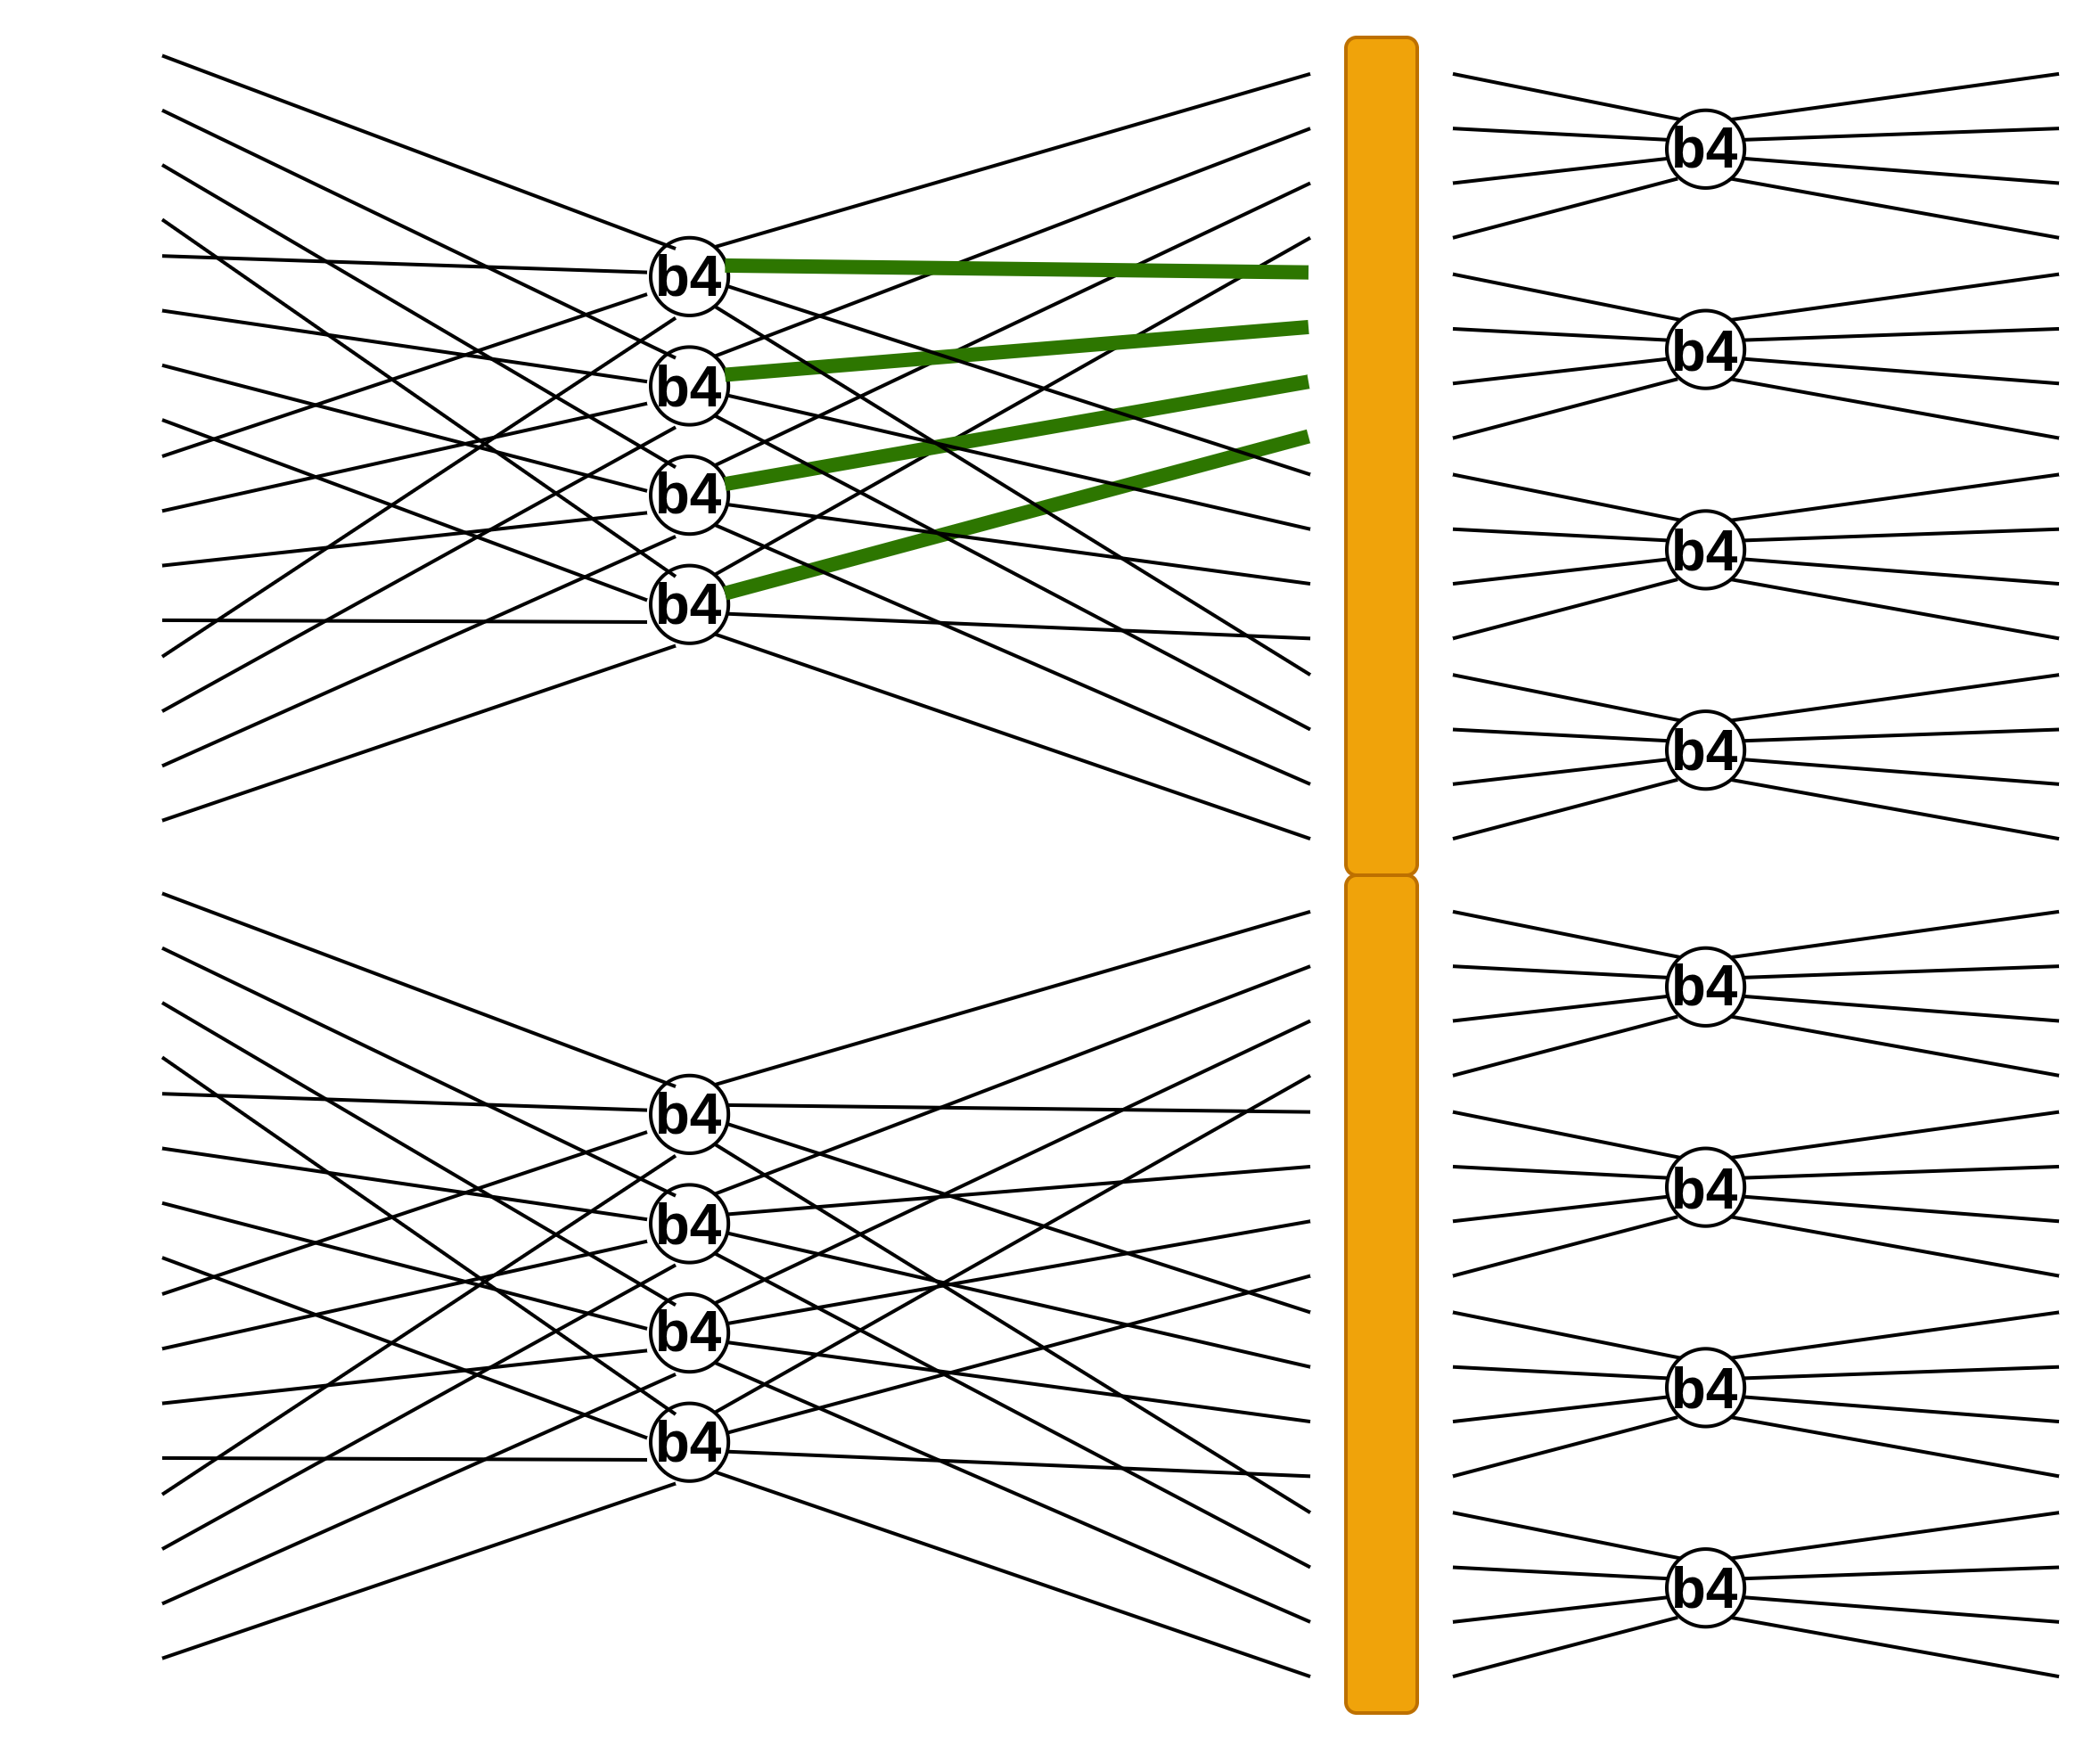
\includegraphics[width=\linewidth]{Images/2nd_tetrada.png}
        \caption{Stride counter equals 01}
        \label{fig:tetrada2}
    \end{subfigure}
    \hfill
    \begin{subfigure}[b]{0.3\linewidth}
        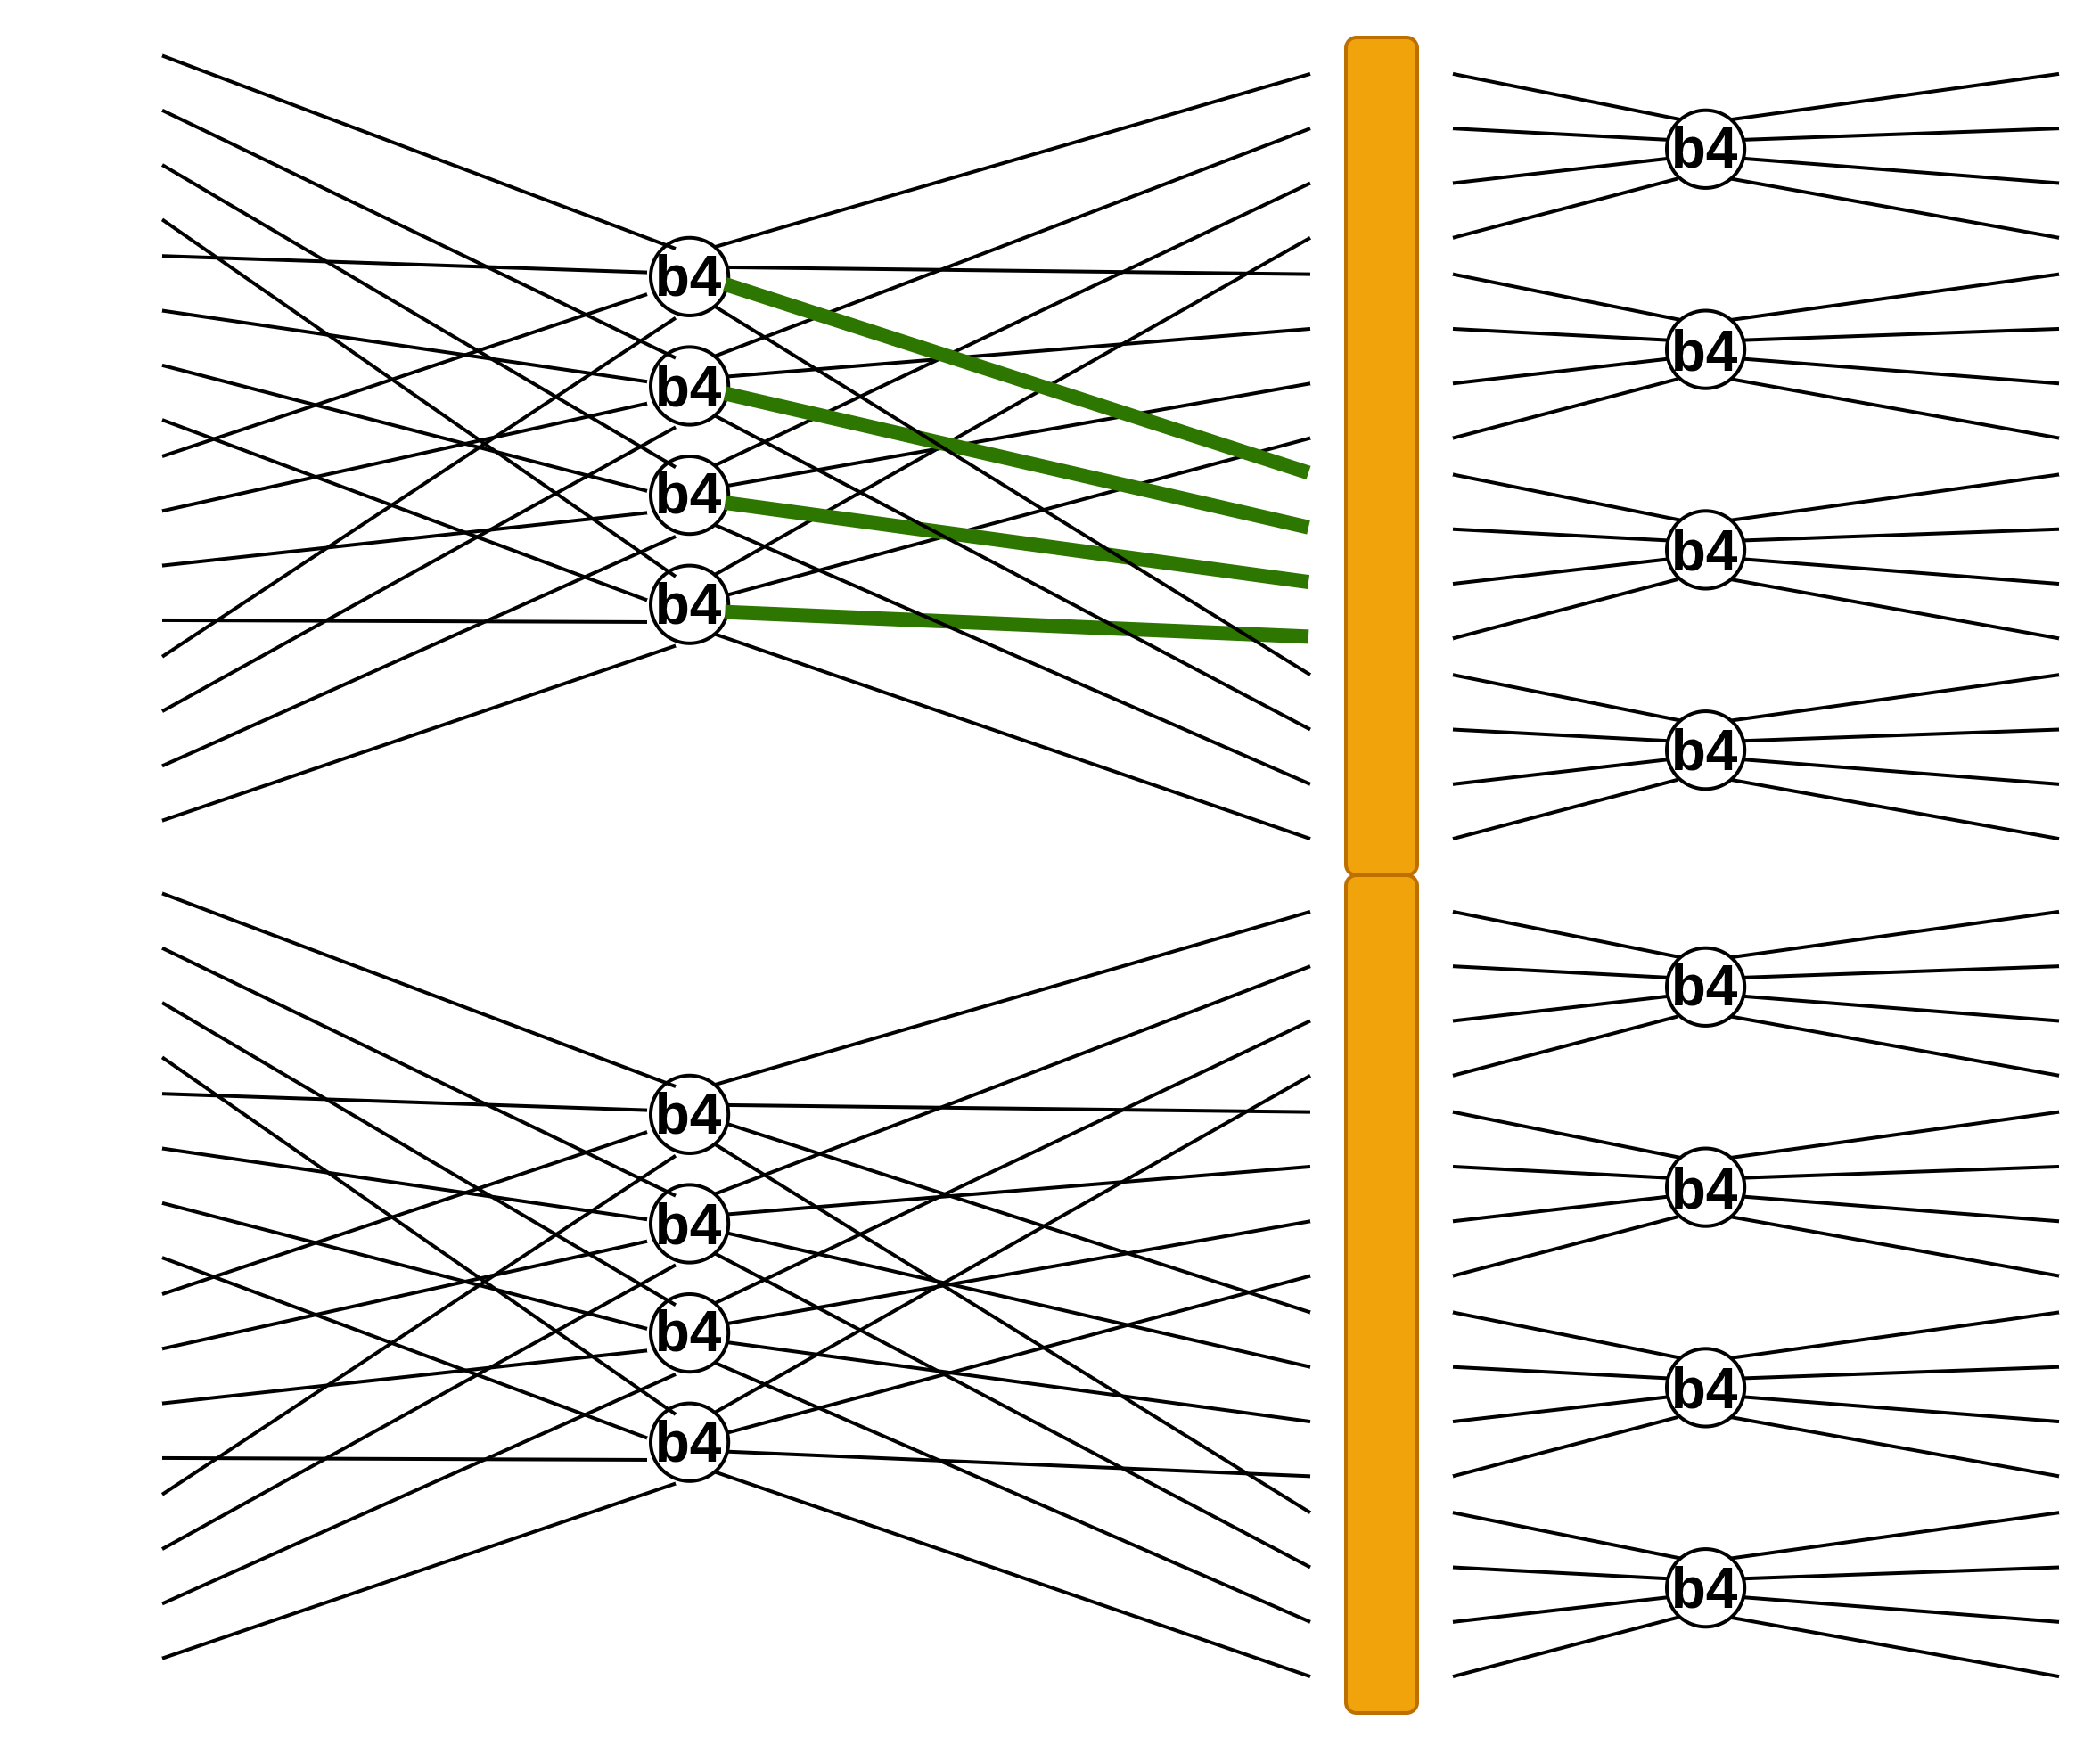
\includegraphics[width=\linewidth]{Images/3rd_tetrada.png}
        \caption{Stride counter equals 10, butterfly counter starts}
        \label{fig:tetrada3}
    \end{subfigure}
    
    \vspace{1em}
    
    % --- Second Row ---
    \begin{subfigure}[b]{0.3\linewidth}
        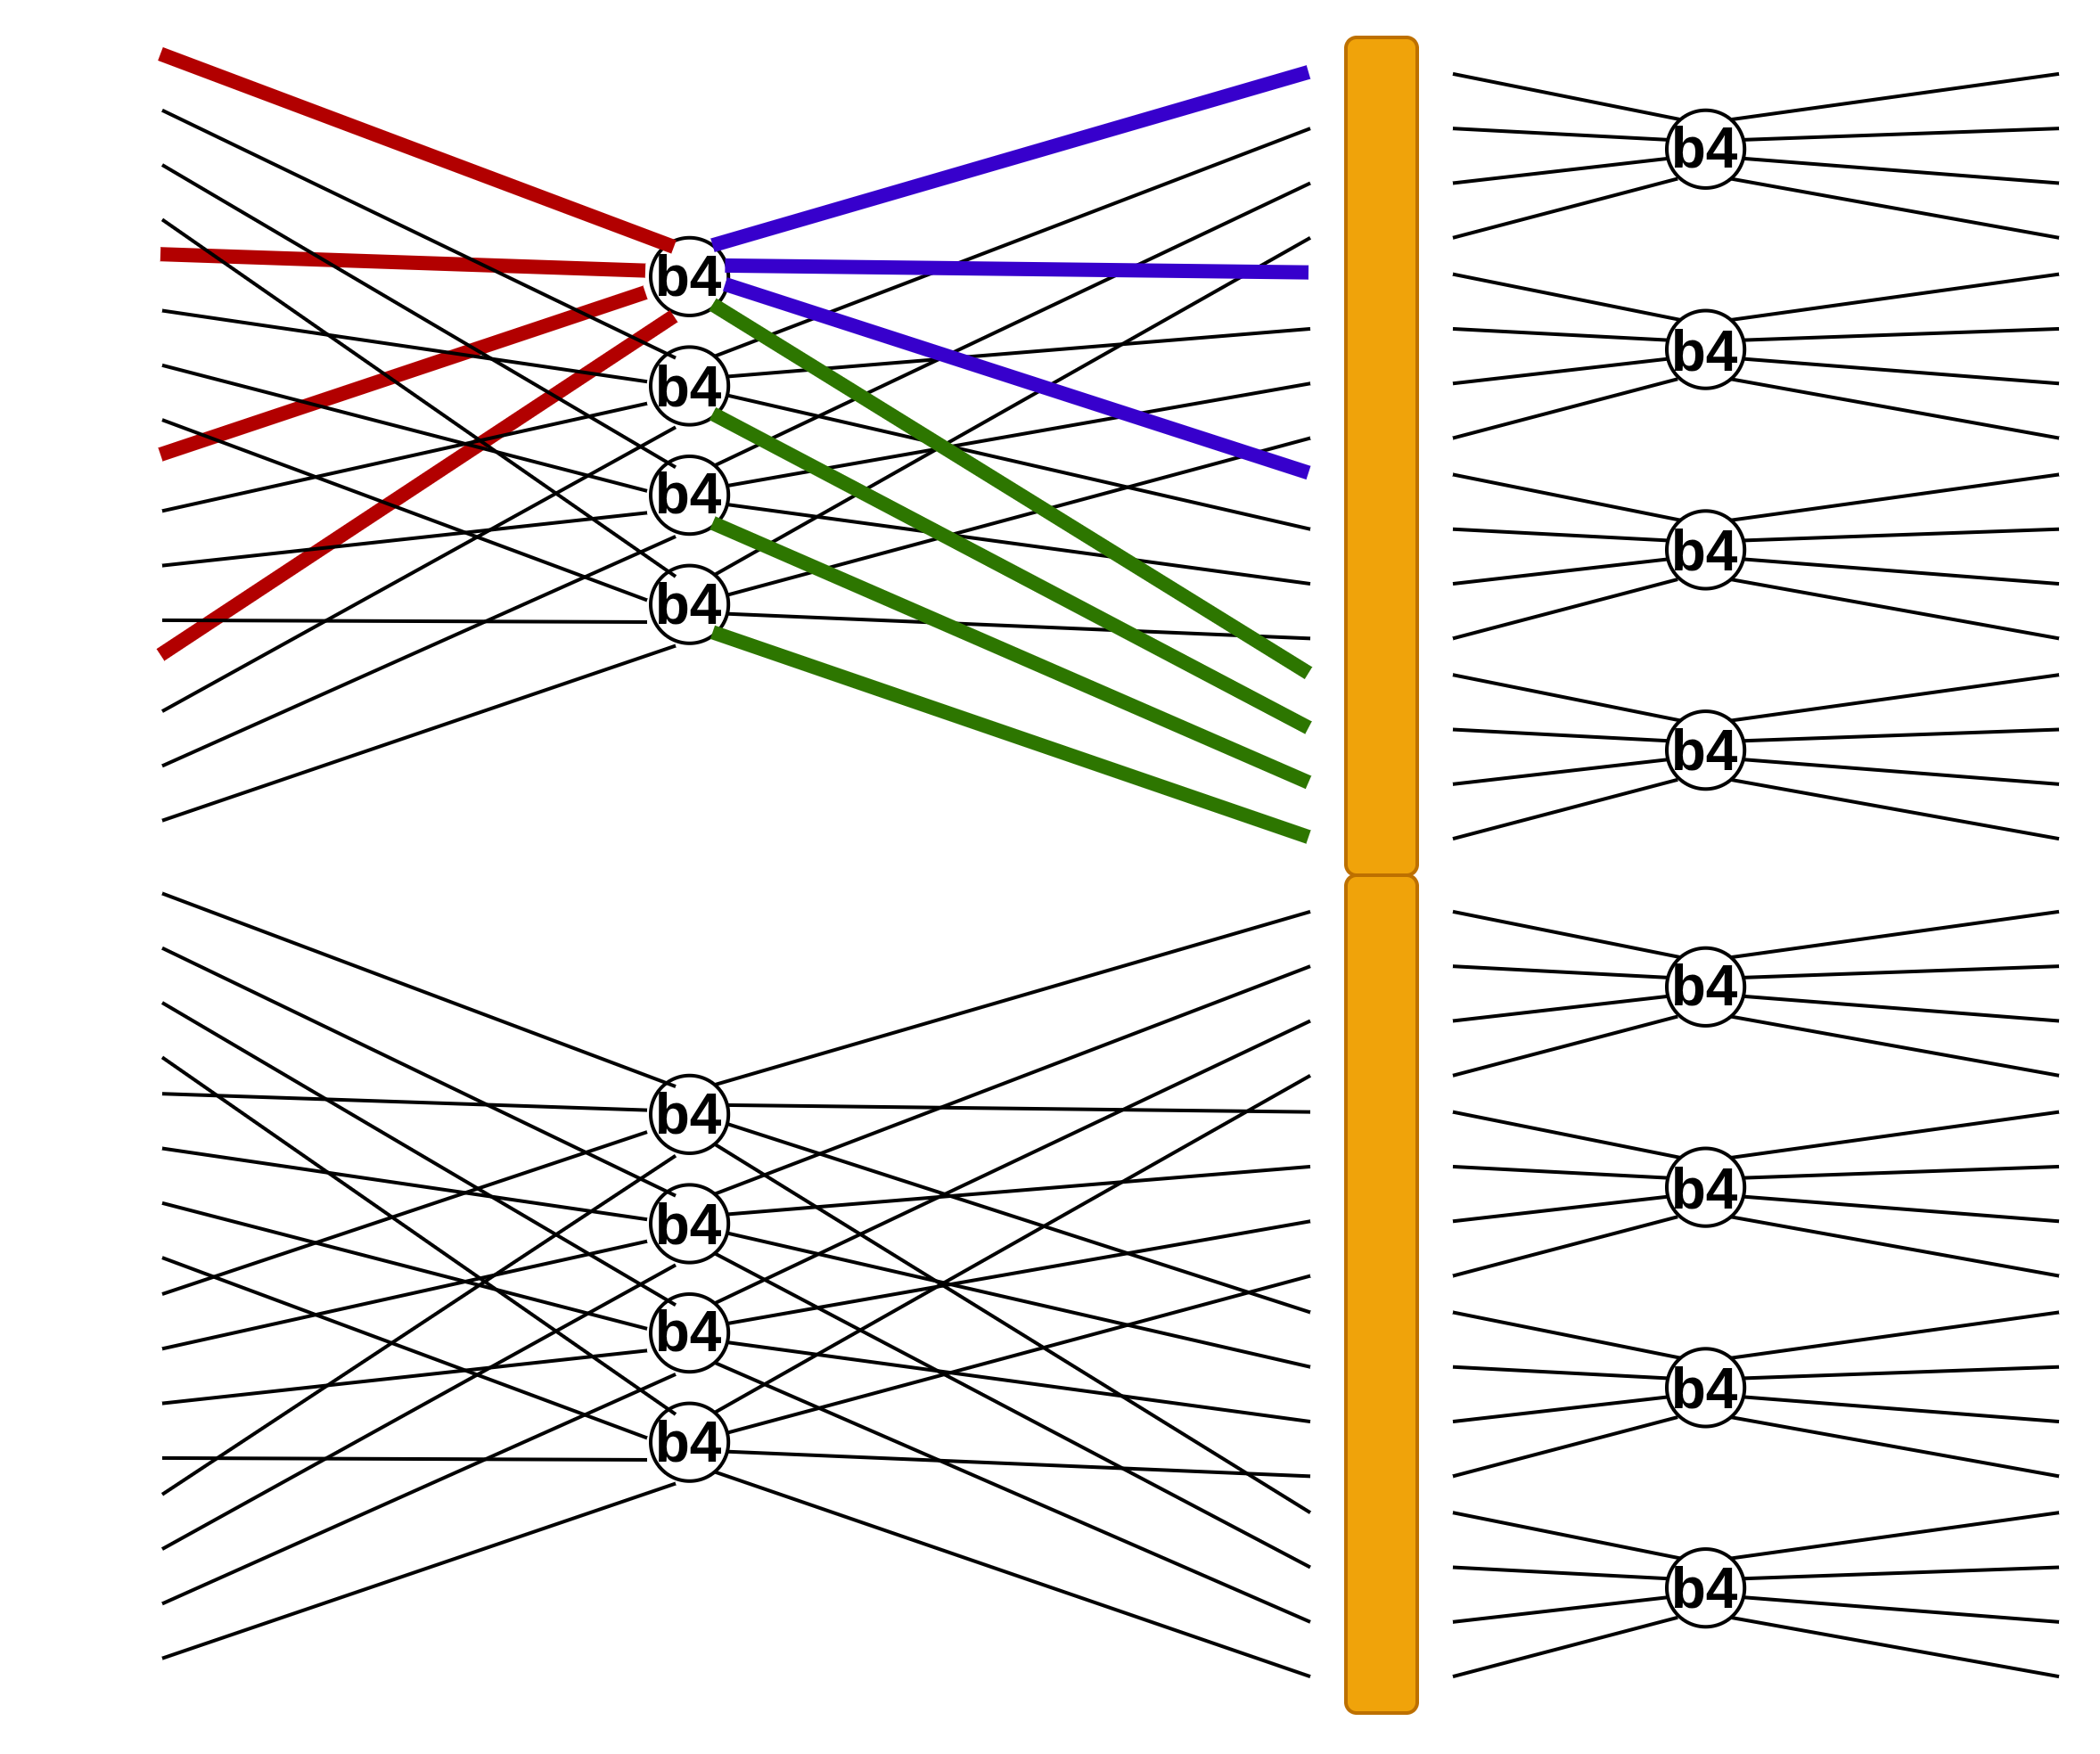
\includegraphics[width=\linewidth]{Images/4th_tetrada.png}
        \caption{Stride counter equals 11, butterfly counter 00}
        \label{fig:tetrada4}
    \end{subfigure}
    \hfill
    \begin{subfigure}[b]{0.3\linewidth}
        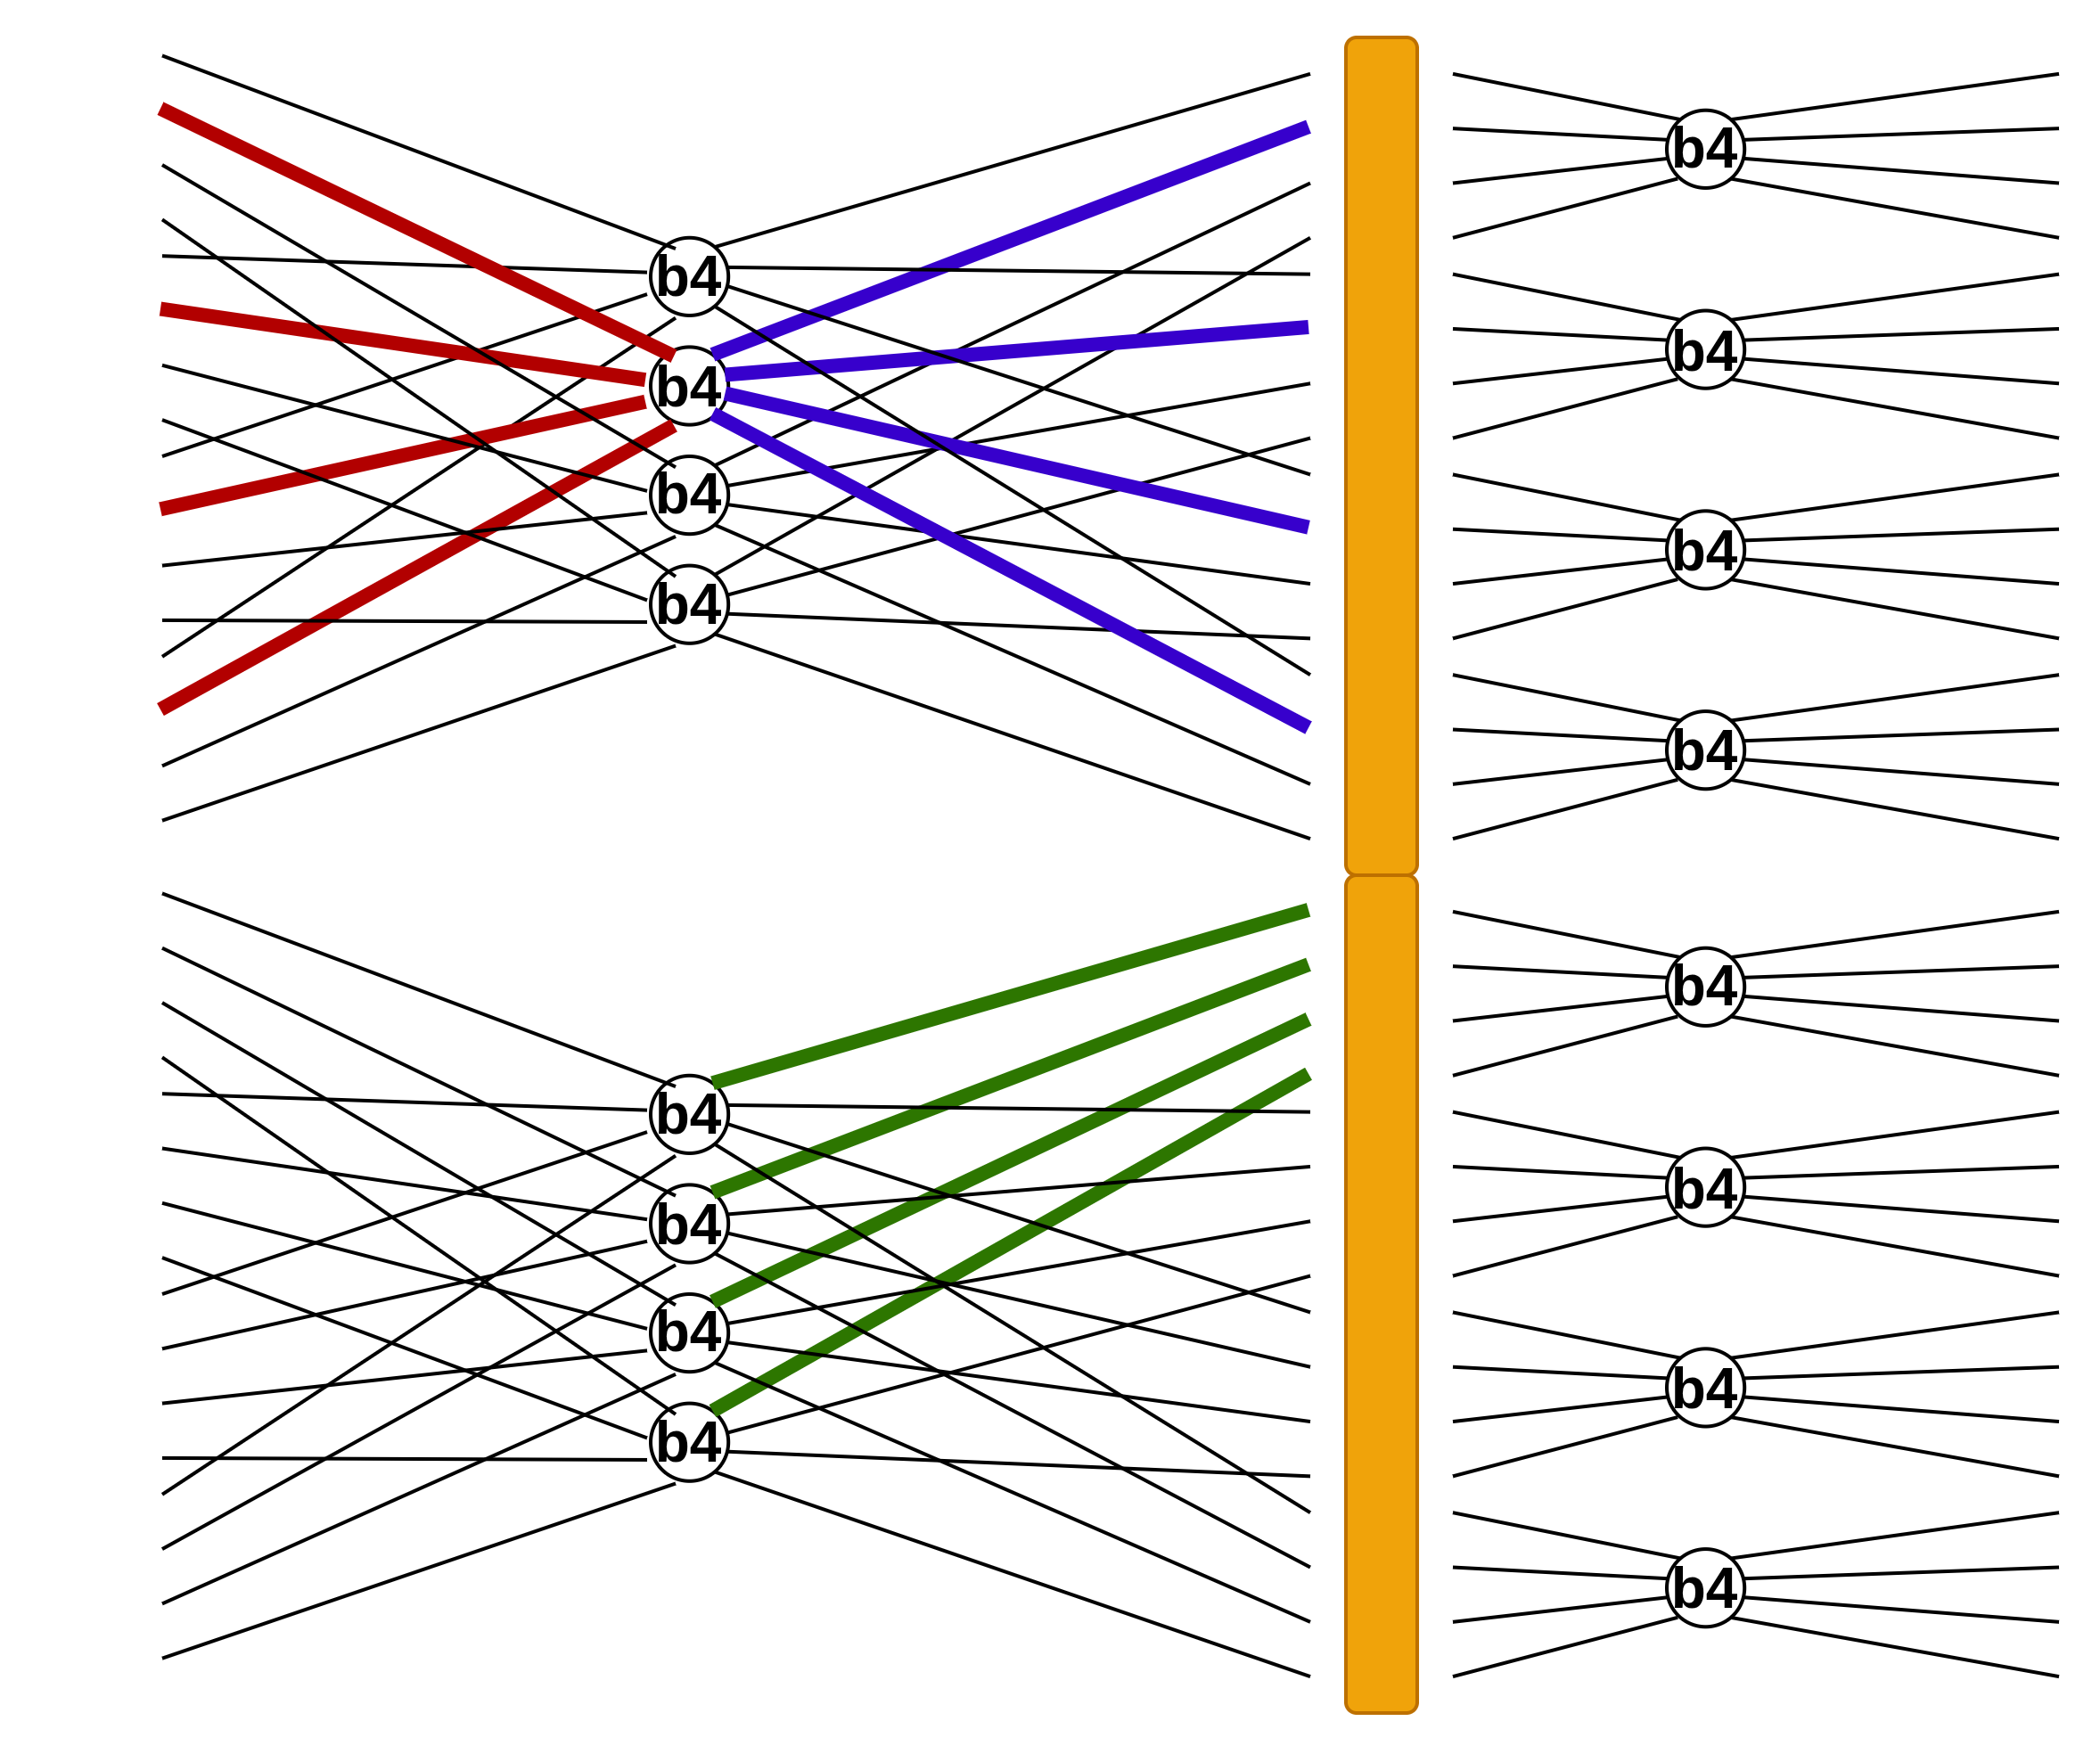
\includegraphics[width=\linewidth]{Images/5th_tetrada.png}
        \caption{Stride counter equals 00, butterfly counter 01}
        \label{fig:tetrada5}
    \end{subfigure}
    \hfill
    \begin{subfigure}[b]{0.3\linewidth}
        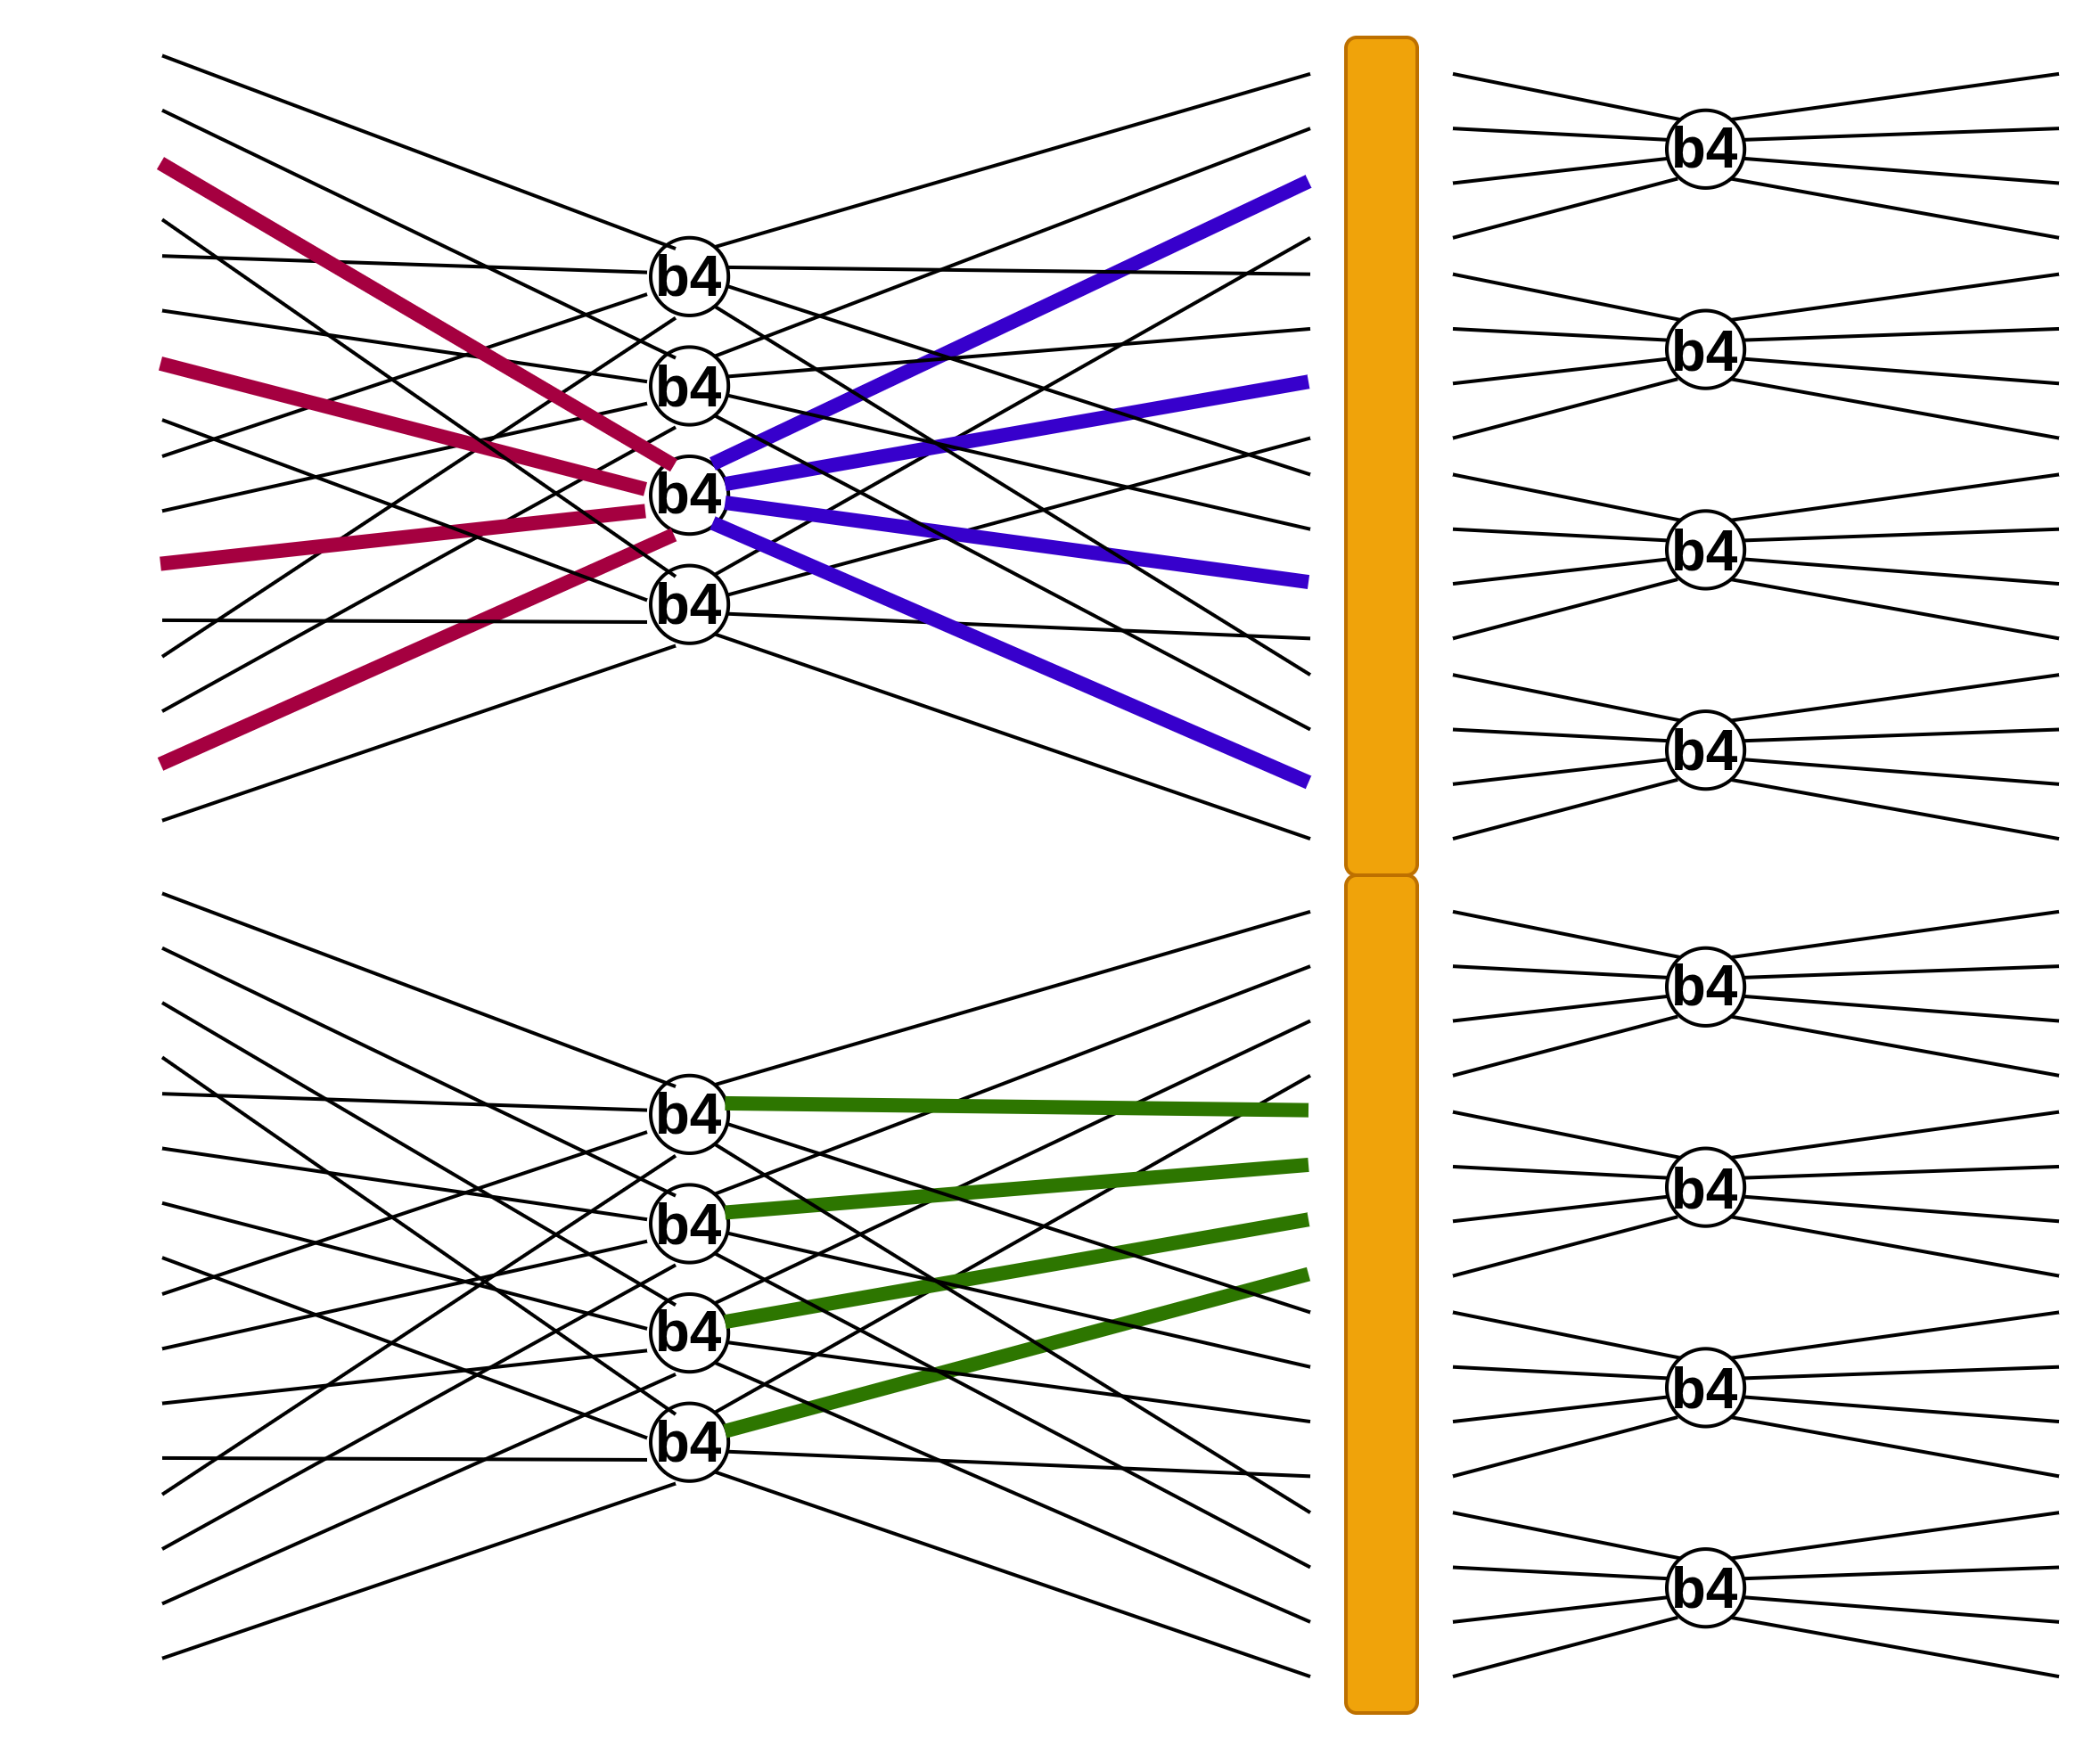
\includegraphics[width=\linewidth]{Images/6th_tetrada.png}
        \caption{Stride counter equals 01, butterfly counter 10}
        \label{fig:tetrada6}
    \end{subfigure}
    
    \caption{Operation flow of the counters managing the sets of four (quads) data points.}
    \label{fig:all_tetradas}
\end{figure}
\subsection{Delay Registers}

\subsection{}

